
\chapter{Formalization}

\def\wf#1{\Vdash #1}

\def\PRName#1{\textsc{I-#1}}
\def\MI{\mathcal{I}}  % prefix rule



In this chapter, we will present the formal proof of the correctness of the language \fmsnesl, a subset of \mysnesl.
First its definition and semantics will be given.
Then \fmsvcode, the target language of \fmsnesl, is defined, and proof of its determinism is given.
The value representation and translation from \fmsnesl to \fmsvcode are also formalized.
Finally we show the proof of the main correctness theorem of this language.

\section{$\mathbf{SNESL_0}$}

The language \fmsnesl we will proof in this chapter is a subset of \mysnesl, with mainly the following simplifications:
\begin{itemize}
	\item only one primitive type $\int$ 
	\item no pairs
	\item selected built-in functions 
	\item restricted comprehension is removed
	\item no user-defined functions
\end{itemize}


\subsection{Syntax}

\noindent (1) The types of \fmsnesl are: 
$$\tau ::= \int \ | \ \tseq{\tau_1}$$

\noindent (2) The synatx of \fmsnesl values : 
$$ n \in \mathbb{Z} $$
$$ v::= n \ | \ \Seqk{v}$$

\noindent (3) The syntax of \fmsnesl expressions and the built-in function are shown in Figure~\ref{fig:fmsnesl-exps}. 
Note that constants can be generated by calling the built-in function $\constn{n}()$ for decreasing expression cases.
Also, the arguments of built-in functions as well as the bound sequence in general comprehension are variables instead of expressions; we can simply convert them into their general forms by adding let-bindings of these variables. 

\fig{
\begin{alignat*}{2}
& e &&::=  x  \tag{variable} \\
&   && \quad | \ \Let{x}{e_1}{e_2} \tag{let-binding}\\
&   && \quad | \ \hcall{\Tupk{x}}  \tag{built-in function call} \\
&   && \quad | \ \Comp{e}{x}{y}{\usevars} \tag{general comprehension} \\
\\
& \hcall && ::= \*{const}_n \ | \ \*{iota} \ | \ \*{plus} 
\end{alignat*}
}{\fmsnesl expressions and built-in functions \label{fig:fmsnesl-exps}}

\subsection{Typing rules}
The typing environment $\Gam$ is a mapping from variables to types: $$\Gamma = [x_1 \|-> \tau_1, ..., x_i \|-> {\tau_i} ]$$
\begin{itemize}
	
	\item Expression typing rules:\\
	
	\Jug{\Type{\Gam}{e}{\tau}}
	
	\PT{
		\AxiomC{}
		\RiLa{(\Gam(x) = \tau)}
		\UC{\Type{\Gam}{x}{\tau}}
	}
	\PT{
		\AC{\Type{\Gam}{e_1}{\tau_1}}
		\AC{\Type{\Gam[x \|-> \tau_1]}{e_2}{\tau}}
		\BC{\Type{\Gam}{\Let{x}{e_1}{e_2}}{\tau}}
	}\\[2ex]
	
	
	\PT{
		\AC{\Typef {\hcall} {\replc{k}{\tau}} {\tau}}
		\RiLa{((\Gam(x_i)= \tau_i)^k_{i=1})}
		\UC{\Type{\Gam}{\hcall{\Tupk{x}}}{\tau}}
	}\\[2ex]
	
	\PT{
		\AC{\Type{[x \|-> {\tau_1}, \j{x_i \|-> \int}]}{e}{\tau}}
		\RiLa{(\Gam(y)=\tseq{\tau_1}, \j{\Gam(x_i) = \int})}
		\UC{\Type{\Gam}{\Comp{e}{x}{y}{\usevars}}{\tseq{\tau}}}
	}\\[2ex]
	
	
\item  Built-in functions typing rules:\\

   \Jug{\Typef {\hcall} {\replc{k}{\tau}} {\tau}}
	
	\PT{\Axiom{\Typef{\constn{n}}{}{\int}}}
	\PT{\Axiom{\Typef{\iotan}{\int} {\tseq{\int}}}}
	\PT{\Axiom{\Typef{\plusn}{\int,\int} {\int}}}
	
	% value types
	\item Value typing rules: \\
	
	\Jug{\TypeV{v}{\tau}}
	
	\PT{\Axiom{\TypeV{n}{\int}}}
	\PT{
		\AC{(\TypeV{v_i}{\tau})^k_{i=1}}
		\UC{\TypeV{\Seqk{v}}{\tseq{\tau}}}
	}
	
\end{itemize}


\subsection{Semantics}
The evaluation environment $\rho$ is a mapping from variables to values: $$ \rho = [x_1 \|-> v_1,...,x_i \|-> v_i]$$ 

\begin{itemize}
\item Expression evaluation rules:
	
	\Jug{\Eval{\rho}{e}{v}}
	\PT{
		\AxiomC{}
		\RiLa{(\rho(x)=v)}
		\UC{\Eval{\rho}{x}{v}}
	}
	\PT{
		\AC{\Eval{\rho}{e_1}{v_1}}
		\AC{\Eval{\rho[x \|-> v_1]}{e_2}{v}}
		\BC{\Eval{\rho}{\Let{e_1}{x}{e_2}}{v}}	
	}\\[2ex]
	
	\PT{
		\AC{\EvalF\hcall{\replc{k}{v}}{v}}
		\RiLa{((\rho(x_i)=v_i)^k_{i=1})}
		\UC{\Eval{\rho}{\hcall{\Tupk{x}}}{v}}
	}\\[2ex]
	
	\PT{
		\AC{(\Eval{[x \|-> {v_i}, \j{x_i \|-> n_i}]}{e}{v_i'})^k_{i=1}}
		\RiLa{(\rho(y)=\Seqk{v}, \j{\rho(x_i) = n_i})}
		\UC{\Eval{\rho}{\Comp{e}{x}{y}{\usevars}}{\Seqk{v'}}}
	}\\[2ex]
	
\item Built-in function evaluation rules:

  \Jug{\EvalF\hcall{\replc{k}{v}}{v}}
	
	\PT{\Axiom{\EvalF{\constn{n}}{}{n}}}
	\PT{\AC{}
		\RiLa{(n \ge 0)}
		\UC{\EvalF{\iotan}{n}{\{0,1,...,n-1\}}}} \\[2ex]
	
	\PT{\AC{} 
		\RiLa{(n_3= n_1+n_2)} 
		\UC{\EvalF{\plusn}{n_1,n_2}{n_3}}}
	
\end{itemize}


\section{$\mathbf{SVCODE_0}$}
The target language of \fmsnesl is also a subset of SVCODE presented in the last chapter. 
We will call it  \fmsvcode.

\subsection{Syntax}
In this minimal language, a primitive stream $\a$ can be a vector of booleans, integers or units, as the following grammar shows:

$$b \in \mathbb{B} = \{\T,\F \}$$
$$ a ::= n \ | \ b \ | \ \unit$$
$$\b = \vrange{b_1}{b_i}$$ 
$$\c = \vrange{()}{()} $$
$$\a = \vrange{a_1}{a_i}  $$ 

\hspace{1cm}

The syntax of \fmsvcode is given in Figure~\ref{fig-svcode-grammar}.


\begin{figure}[H] \large
	\begin{alignat*}{2}
	&p  && :: = \ \epsilon \\ 
	&   &&\ \ | \ \sdef{\s}{\psi(s_1,...,s_k)} \\
	&   &&\ \ | \ \withctrl{\s}{p_1}{\Sin}{\Sout} \\
	&   &&\ \ | \ p_1;p_2  \\
	\\
	&\s && ::= 0 \ | \ 1 \ ... \in \SId  = \mathbb{N}   \tag{stream ids}\\
	\\
	& \psi \ && ::= \consta{a} \ | \ \toflag  
	\ | \ \usum \ | \ \maptwo{\oplus} \ | \ \scan_{n_0} \ | \ \distr  \tag{Xducers} \\
%	& \oplus \ && :: = + \ | \ - \ | \ \times \ | \ \div \ | \ \% \ | \ \le \ | \ ...  \tag{binary operations}\\
	\\
	&  \S && ::= \{\s_1,..., \s_i\} \in \sset  \tag{a set of stream ids}
	\end{alignat*}
	\caption{Abstract syntax of \fmsvcode \label{fig-svcode-grammar}}
%TODO fix Xducer maptwo?
\end{figure}


The function $\texttt{dv}$ returns the set of defined variables of a given \fmsvcode program.

\begin{alignat*}{2}
&\dv{\epsilon} && =  \emptyset \\
&\dv{\sdef{\s}{\psi(s_1,...,s_k)}} && =  \{s\} \\
&\dv{\withctrl{\s_c}{p_1}{\Sin}{\Sout}} && =   \Sout \\
&\dv{p_1;p_2} && =  \dv{p_1} \cup \dv{p_2} \\
\end{alignat*}

Correspondingly, $\texttt{fv}$ returns the free variables set.

\begin{alignat*}{2}
&\FV{\epsilon} && = \emptyset \\
&\FV{\sdef{\s}{\psi(s_1,...,s_i)}} && = \{s_1,...,s_k\}\\
&\FV{\withctrl{\s_c}{p_1}{\Sin}{\Sout}} && = \{s_c\} \cup \Sin \\
&\FV{p_1;p_2} && = \FV{p_1} \cup (\FV{p_2} - \dv{p_1}) \\
\end{alignat*}


An immediate property of this language is that the defined variables of a \emph{well-formed} \fmsvcode program are always fresh. In other words, there is no overlapping between the free variables and the newly generated ones.

\begin{defi}[\textbf{Well-formedness}]
	p is a well-formed SVCODE program, written as $\Vdash p$, if one of the following rules applies:
\end{defi}
  \Jug{\wf{p}}
	
	\PT{\Axiom{\wf{\epsilon}}}
    \PT{ \RiLa{(s\notin \{s_1,...,s_k\})}
   		\Axiom{\wf{\sdef{s}{\lcall(s_1,...,s_k)}}}}\\[3ex]
   	
   	\PT{\AC{\wf{p_1}}
    	\RiLa{\left(
    		\begin{aligned}
    			&\FV{p_1} \subseteq \Sin \\
    			&\Sout \subseteq \dv{p_1} \\
    			&(\{\s\} \cup \Sin)  \cap \dv{p_1} = \emptyset
    		\end{aligned}
    		 \right)} 
    	\UC{\wf{\withctrl{s}{p_1}{\Sin}{\Sout}}}  
   	}\\[3ex]
   
   \PT{\AC{\wf{p_1}}
   	   \AC{\wf{p_2}}
   	   \RiLa{\left(
   	   	\begin{aligned}
   	   		(\FV{p_1} \cup \dv{p_1}) \cap \dv{p_2} = \emptyset \\
   	   	\end{aligned}
      	\right)}  	  
       \BC{\wf{(p_1;p_2)}}
   }\\[3ex]
   


\begin{lem}[\textbf{Freshness}]
	If $p$ is well-formed, then  $\FV{p} \cap \dv{p} = \emptyset $. 
\end{lem}

The proof is straightward by induction on the derivation of $\wf{p}$.

%TODO well-formed 

\subsection{Instruction semantics}

Before showing the semantics, we first introduce some notations and operations about streams for convenience.
\begin{nota}
	Let $\< a_0 | \a \'>$ denote a non-empty stream $\< a_0,a_1,...,a_i \'>$ for some $\a = \< a_1,...,a_i \'>$. 
\end{nota}


\begin{nota}[\textbf{Stream concatenation}]
	$\vapp{\vrange{a_1}{a_i}} {\vrange{a_1'}{a_j'}} = \langle a_1,...,a_i,a_1',...,a_j' \rangle $ \\
	
\end{nota}

The operational semantics of \fmsvcode is given in Figure~\ref{fig-svcode-semantics}.
The runtime environment or store $\sgm$ is a mapping from stream variables to vectors:
$$\sgm = [\s_1 \|-> {\a_1},...,\s_i \|-> {\a_i}]$$
The control stream $\c$, which is basically a vector of units representing an unary number, indicates the $parallel \ degree$ of the computation. 
It is worth noting that only in the rule $\PName{Wc-Nonemp}$ the control stream has a chance to get changed.


\begin{figure}[H]\large 
	
	\Jug{\seval{p}{\sgm}{\c}{\sgm'}}\\
	
	
	\PT{\LeLa{\PName{Empty:}}  \Axiom{{\seval{\epsilon}{\sgm}{\c}{\sgm}}{}}} \\[2ex]
	
	\PRule{Xducer}{\PT{\AC{\sevalf{\a_1}{\a_k}{\c}{\a}}
			\RiLa{((\sgm(\s_i) = \a_i)^k_{i=1})}
			\UC{\seval{\sdef{\s}{\lcall\Tupk\s}}{\sgm}{\c}{\sgm[\s \|-> \a]}}
	}} \\[4ex]
	
	\PT{ \LeLa{\PName{Wc-Emp:}}
		\AC{}
		\RiLa{
			\left(
			\begin{aligned}
				&\forall s \in \{s_c\} \cup \Sin. \sgm(s) = \emptyv \\
				&\Sout = \{s_1,...,s_l\}
			\end{aligned}
			\right)}
		\UC{\seval{\withctrl{\s_c}{p_1}{\Sin}{\Sout}}{\sgm}{\c}{\sgm[\l{\s_i \|-> \emptyv}]}}
	}\\[2ex]
	\PRule{Wc-Nonemp}{\PT{
			\AC{\seval{p_1}{\sgm}{\c_1}{\sgm''}}
			\RiLa{\left(
				\begin{aligned} 
					&\sgm(\s_c)= \c_1 \ne \emptyv \\
					&\Sout = \{s_1,...,s_l\}
				\end{aligned}\right)}
			\UC{\seval{\withctrl{\s_c}{p_1}{\Sin}{\Sout}}{\sgm}{\c}{\sgm[\l{\s_i \|-> \sgm''(\s_i)}]}}
	}}\\[4ex]
	
	\PRule{Seq}{\PT{
			\AC{\seval{p_1}{\sgm}{\c}{\sgm''}}
			\AC{\seval{p_2}{\sgm''}{\c}{\sgm'}}	
			\BC{\seval{p_1;p_2}{\sgm}{\c}{\sgm'}}
	}}
	
	\caption{\fmsvcode semantics}
	\label{fig-svcode-semantics}
\end{figure}

The rule $\PName{Empty}$ is trivial, empty program doing nothing on the store. 

The rule $\PName{Xducer}$ adds the store a new stream binding where the bound vector is generated by a specific Xducer. The detailed semantics of Xducers are defined in the next subsection. 

The rules $\PName{Wc-Emp}$ and $\PName{Wc-Nonemp}$ together show two possibilities for interpreting a \wc instruction:
\begin{itemize}
	\item if the new control stream $\s_c$ and the streams in $\Sin$, which includes the free variables of $p_1$, are all empty, then just bind empty vectors to the stream ids in $\Sout$, which are part of the defined streams of $p_1$.
	\item otherwise execute the code of $p_1$ as usual under the new control stream, ending in the store $\sgm''$; then copy the bindings of $\Sout$ from $\sgm''$ to the initial store. 
\end{itemize}

\subsection{Xducer semantics}
The semantics of Xducers are abstracted into two levels: the $general$ level and the $block$ level. The general level summarizes the comman property that all Xducers share, and the block level describes the specific behavior of each Xducer. 

Figure~\ref{fig-xducer-semantics} shows the semantics at the general level. 


\begin{figure}[H]\large
	
	\Jug{\sevalf{\a_1}{\a_k}{\c}{\a}} \\
		
	\PRule{X-Loop}{\PT{
			\AC{\block{\a_{11}}{\a_{k1}}{\a_{01}}}
			\AC{\sevalf{\a_{12}}{\a_{k2}}{\c_0}{\a_{02}}}
			\RiLa{((\vapp{\a_{i1}}{\a_{i2} = \a_i})^k_{i=0})}
			\BC{\sevalf{\a_1}{\a_k}{\< () | \c_0 \rangle}{\a_0}}
	}}\\[4ex]
	
	\LeLa{\PName{X-Termi:}} 
	\Axiom{\sevalf {\emptyv_1} {\emptyv_k} \emptyv \emptyv}
	\DisplayProof \footnotemark	
	\caption{General semantics of \fmsvcode Xducers \label{fig-xducer-semantics}}
\end{figure}
\footnotetext{For notational convenience, in this thesis we add subscripts to a sequence of constants, such as $\emptyv, \F, 1$, to denote the total number of these constants.}

There are only two rules for the general semantics. 
They together say that the output stream is computed in a ``loop" fashion, where the 
iteration uses specific block semantics of the Xducer and the number of iteration is the unary number that the control stream represents, i.e., the length of the control stream. 
In the parallel setting, we prefer to call this iteration a $block$. 
Recall the control stream is a representation of the parallel degree of the computation, then a block consumes exact one degree. 
It it worth noting that all these blocks are data-independent, which means they can be executed in parallel. 
So the control stream indeed carries the theoretical
maximum number of processors we need to execute the computation most efficiently, if the computation within the block cannot be parallelized further. \\


After abstracting the general semantics, the remaining work of formalizing the specific semantics of Xducers within a block becomes relatively clear and simple. The block semantics are defined in Figure~\ref{fig:xducer-bl-seman}. 

\begin{figure}[H]\large
	\def\'>{\rangle}
	
	\Jug{\block{\a_1}{\a_k}{\a}} \\
	
	\PT{\LeLa{\PName{X-Const:}} 
		\Axiom{\blockf{\consta{a}}{}{\singl{a}}}
	}
	\PT{\LeLa{\PName{X-ToFlags:}} 
		\Axiom{\blockf{\toflag}{\singl{n}}{\< \F_1,...,\F_n,\T \'>}} } \\[3ex]
	\PRule{X-MapTwo}{\PT{\AC{}
			\RiLa{(n_3= n_1 \oplus n_2)}
			\UC{\blockf{\maptwo{\oplus}}{\singl{n_1}, \singl{n_2}} {\singl{n_3}}}
	}} \\[3ex]
	
	%--- UsumF
	\PRule{X-UsumF}{
		\PT{\AC{\blockf{\usum}{\b}{\a}}
			\UC{\blockf{\usum}{ \<\F|\b \'>}{\<()|\a\'>}}
		}
	}
	\PT{\LeLa{\PName{X-UsumT:}} \Axiom{\blockf{\usum}{\oT}{\emptyv}}}
	\\[3ex]

	\PRule{X-ScanF}{
		\PT{\AC{\blockf{\scan_{n_0+n}}{\b,\a}{\a'}}
			\UC{\blockf{\scan_{n_0}}{\<\F|\b \'>, \<n|\a\'>}{\<n_0|\a'\'>}}
		}		
	}\\[3ex]

	\PT{\LeLa{\PName{ScanT:}} 
		\Axiom{\blockf{\scan_{n_0}}{\oT, \emptyv}{\emptyv}}
	}\\[3ex]
		
	\PRule{X-DistrF}{
		\PT{\AC{\blockf{\distr}{\b, \<n\'>}{\a}}
			\UC{\blockf{\distr}{\<\F|\b \'>, \<n\'>}{\<n|\a \'>}}
		}
	}
	\PT{\LeLa{\PName{X-DistrT:}}\Axiom{\blockf{\distr}{\oT,\<n\'>}{\emptyv}}}\\[1ex]
		
\caption{Block semantics of  Xducers \label{fig:xducer-bl-seman}}
\end{figure}



%\begin{itemize}
%	\renewcommand{\labelitemi}{$-$}
%	\item $\constaf{a}$ outputs the const $a$ until the control stream reaches EOS.
%	
%	\begin{example} \emph{$\constaf{3}$ with control stream $\c = \<(),()\'>$:}\\
%		\begin{center}
%			
\includegraphics[width=0.6\textwidth]{fig/const3.png}
%		\end{center}
%	\end{example}
%	
%	\item $\toflagf{\singl{n}}$ first outputs $n$ $\F$s, then one $\T$.
%	
%	\begin{example} \emph{$\toflagf{\<2,0\'>}$:}\\
%		\begin{center}
%			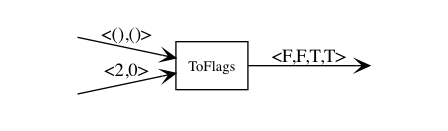
\includegraphics[width=0.6\textwidth]{fig/toflag.png}
%		\end{center}
%	\end{example}
%	
%	\item $\maptwof{\oplus}{\singl{n_1}}{\singl{n_2}}$ outputs 
%	the binary operating result of $\oplus$ on $n_1$ with $n_2$. 
%	
%	\begin{example} \emph{$\maptwof{+}{\<3,2\'>}{\<1,1\'>}$:}\\
%		\begin{center}
%			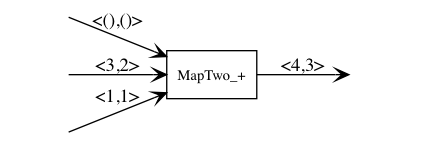
\includegraphics[width=0.6\textwidth]{fig/maptwo.png}
%		\end{center}
%	\end{example}
%	
%	
%	
%
%\end{itemize}
%



As have discussed before, we consider a block  as the minimum computing unit assigned to a single processor. This is reasonable for
Xducers such as $\consta{a}$ and $\maptwo{\oplus}$, because
they are already sequential at the block level. 

However, some other Xducers, such as $\usum$, can be parallelized further inside a block.
As we extend the language with more Xducers, we could find that computations on unary numbers within blocks are common, which is mainly due to the value representation strategy we use, but also more difficult to be regularized.
For the scope of this thesis, the block semantics we have shown are already relatively clear and simple enough to reason about, and the unary level parallelism can be investigated in future work. 



%Or if we want to use $unary$ semantics maybe for later: \\
%\begin{mdframed}
%\PT{
%	\AC{\unary{\singl \F}{\a_{k1}}{\a_1}}
%	\AC{\block{\a_{12}}{\a_{k2}}{\a_2}}
%	\RiLa{(\a = \vapp{\a_1}{\a_2})}
%	\BC{\block{\vapp {\singl\F} {\a_{12}}} {\vapp {\a_{k1}} {\a_{k2}}}{\a}}
%}\\[2ex]
%
%\PT{
%	\AC{\unary{\oT} {\a_k}{\a}}
%	\UC{\block{\oT}{\a_k} \a}
%}\\[2ex]
%
%\begin{itemize}
%\item Transducer $unary$ semantics:\\ 
%
%\Jug{\unary{\singl b}{\a_k}{\a}}
%
%\PT{ \Axiom{\usum(\oF) \dda \vunit}}
%\PT{\Axiom{\usum(\oT) \dda \emptyv }} \\[1ex]
%
%
%%loopuv
%\item Transducer block with $accumulator$: \\
%
%\Jug{\blockv{n}{\a_1}{\a_k}{\a}}
%\PT{
%	\AC{\unaryv{n_0} {\singl \F}{\a_{k1}}{n_0'} {\singl{n_1}}  }
%	\AC{\blockv{n_0'}{\a_{12}}{\a_{k2}}{\a_2}}
%	\BC{\blockv{n_0} {\vapp {\singl\F} {\a_{12}}} {\vapp {\a_{k1}} {\a_{k2}}}{\vapp {\singl{n_1}} {\a_2}} }
%}\\[2ex]
%
%\PT{
%	\AC{\unaryv {n_0} \oT {\a_k} {} {\a}}
%	\UC{\blockv {n_0} \oT {\a_k} {\a} }
%}
%
%\item Transducer unary with $accumulator$: \\
%
%\Jug{\unaryv{n}{\oF}{\a_k}{n'}{\a}}
%
%\PT{\Axiom{\scan_{n_0}(\oF,{\singl{n}}) \dda^{n_0+n} {\singl{n_0}} }} \\
%
%\Jug{\unaryv{n}{\oT}{\a_k}{}{\a}}
%
%\PT{\Axiom{\scan_{n_0}(\oT, \emptyv) \dda {\emptyv} }}
%\end{itemize}
%\end{mdframed}

\subsection{$\mathbf{SVCODE_0}$ determinism}

We now present  how we prove a well-formed \fmsvcode program is deterministic.\\

\begin{defi}[\textbf{Stream prefix}]
	$\a$ is a $prefix$ of $\a'$, written $\a \prefix \a'$, if one of the following rules applys: \\
	
	\emph{\Jug{\a \prefix \a'}}
	\PT{\LeLa{\PRName{Emp:}} \Axiom{\emptyv \prefix \a' }}
	\PRName{Nonemp:}{
		\PT{
			\AC{\a \prefix \a'}
			\UC{\<a_0 \ | \ \a \'> \prefix \<a_0 \ | \ \a' \'>}
	}}\\
	
\end{defi}

\begin{lem}\label{lem-app2pre}
	If $\a_1 {\++} \a_2 = \a$, then $\a_1 \prefix \a$.
\end{lem}
\begin{proof}
	The proof is straightforward by induction on $\a_1$: case $\a_1 = \emptyv$ and case $ \a_1 = \< a_0 \ | \ \a_1' \'>$ for some $\a_1'$.
\end{proof}

The following lemma says that a Xducer always knows how many elements it should consume and produce when it reads one element from the control stream, i.e., for one block, and these numbers are fixed in any block for the same Xducer.


\begin{lem}[\textbf{Blocks are self-delimiting}] \label{lem-block-unique}
	If
	\begin{enumerate}[(i)]
		\item $(\a_i' \prefix  \a_i \ by \ some \ derivation \ \MI_{i})^k_{i=1}$ and $\block{\a_1'}{\a_k'}{\a'}$ by some $\MP$, 
		\item $(\a_i'' \prefix \a_i \ by \ some \ derivation \ \MI'_{i})^k_{i=1}$ and
		$\block{\a_1''}{\a_k''}{\a''}$ by some $\MP'$.
	\end{enumerate} 
	then \begin{enumerate}[(i)]
		\item $(\a_i' = \a_i'')^k_{i=1}$ 
		\item $\a' = \a''$.
	\end{enumerate}
\end{lem}

\begin{proof}
	The proof can be done by induction on $\MP$. We show three cases 
	$\PName{-X-ToFlags}$, $\PName{-X-ScanT}$ and $\PName{-X-ScanF}$ here; the others are analogous.
	\begin{itemize}
		\item Case $\MP$ uses $\PName{-X-ToFlags}$. \\
		Then
		$$	\PT{\LeLa{\MP =} 
			\Axiom{\blockf{\toflag}{\singl{n_1}}{\< \F_1,...,\F_{n_1},\T \'>}} }
		$$
		and 
		$$	\PT{\LeLa{\MP' =} 
			\Axiom{\blockf{\toflag}{\singl{n_2}}{\< \F_1,...,\F_{n_2},\T \'>}} }
		$$
		so $k=1, \a_1' = \singl{n_1}$, $\a' = \< \F_1,...,\F_{n_1},\T \'>$, and  
		$\a_1'' = \singl{n_2}$, $\a'' = \< \F_1,...,\F_{n_2},\T \'>$. \\
		Since both $\a_1'$ and $\a_1''$ are nonempty, $\MI_{1}$ and $\MI_{1}'$ must both use the rule $\PRName{Nonemp}$,
		which implies $n_1$ = $n_2$. 
		Then it is clear that $\a_1' = \a_1''$ and $\a' = \a''$, as required. 
		
		\item Case $\MP$ uses $\PName{-X-ScanT}$. \\
		Then 	
		$$\PT{\LeLa{\MP = } \Axiom{\blockf{\scan_{n_0}}{\oT, \emptyv}{\emptyv}}}$$
		so $k$=2, $\a_1' = \oT$. 
		Since $\a'_1$ is nonempty, then $\MI_{1}$ must use $\PRName{Nonemp}$, which implies the first element of $\a_1$ is $\T$. \\		
		There are two possibilities for $\MP'$:
		\begin{itemize}
			\item Subcase $\MP'$ uses $\PName{-X-ScanF}$.\\
			This subcase is impossible, because it requires $\a_1$ starts with a $\F$, which is contradictory to what we already know.
			
			\item Subcase $\MP'$ uses $\PName{-X-ScanT}.$ \\
			Then $$\PT{\LeLa{\MP' = } \Axiom{\blockf{\scan_{n_0}}{\oT, \emptyv}{\emptyv}}}$$
			So $\a''_1 = \oT = \a'_1$, $\a''_2 = \emptyv = \a'_2$, and $\a'' = \emptyv = \a''$, as required. 
			
		\end{itemize}
		
		
		\item Case $\MP$ uses $\PName{-X-ScanF}$. \\
		Then 
		$$\PT{\UCN{\MP_0}{\blockf{\scan_{n_0+n}}{\a'_{10},\a'_{20}}{\a_0'}}
			\LeLa{\MP = }
			\UC{\blockf{\scan_{n_0}}{\<\F|\a'_{10} \'>, \<n|\a'_{20}\'>}{\<n_0|\a'_0\'>}}
		}$$
	
		So $k$=2, $\a_1' = \<\F|\a'_{10} \'>$, and $\a_2' = \<n|\a'_{20}\'>$. 
		$\MI_{1}$ must use $\PRName{Nonemp}$, which implies the first element of $\a_1$ is $\F$. So $\a_1 = \< \F | \a_{10}\'>$ for some $\a_{10}$. 
		By the rule $\PRName{Nonemp}$, we have
			$$\PT{
				\AC{\a'_{10} \prefix \a_{10}}
				\UC{\<\F|\a'_{10} \'> \prefix \< \F | \a_{10}\'>}
			}$$
				
		Similarly, we can assume  $\a_2 = \<n |\a_{20} \'>$, and we must have $\a'_{20} \prefix \a_{20}$.
		Thus, \eq{eq-scan-determ-1}{
			( \a_{i0}' \prefix \a_{i0} )^2_{i=1}}
		There are two possibilities for $\MP'$:
		\begin{itemize}
			\item Subcase $\MP'$ uses $\PName{-X-ScanT}$.\\
			This subcase is impossible, because $\a_1$ does not start with a $\T$. 
			
			\item Subcase $\MP'$ uses $\PName{-X-ScanF}$.\\
			Then	
			$$\PT{\UCN{\MP_0'}{\blockf{\scan_{n_0+n}}{\a''_{10},\a''_{20}}{\a''_0}}
				\LeLa{\MP' = }
				\UC{\blockf{\scan_{n_0}}{\<\F|\a''_{10} \'>, \<n|\a''_{20}\'>}{\<n_0|\a''_0\'>}}
			}$$
			so $\a_1'' =  \<\F|\a''_{10} \'>, \a_2'' = \<n|\a''_{20}\'>$, $\a'' = \<n_0|\a''_0\'>$, 
			and it is easy to show  \eq{eq-scan-determ-2}{
				(\a''_{i0} \prefix \a_{i0} )^2_{i=1}}
			
			Here we first prove the following inner lemma: \\		
			if $(\a'_{i0} \prefix \a_{i0} )^2_{i=1}$ and $\blockf{\scan_{n_0}}{\a'_{10},\a'_{20}}{\a'}$ by some derivation $\MP_0$,
		    $(\a''_{i0} \prefix \a_{i0} )^2_{i=1}$ and $\blockf{\scan_{n_0}}{\a''_{10},\a''_{20}}{\a''}$,
			then $\a'_{10} = \a''_{10}, \a'_{20} = \a''_{20}$,  and $\a' = \a''$. \\
			The proof is by induction on $\MP_0$.  There are two subcases:
			for the case $\MP_0$ uses $\PName{-X-ScanT}$, the proof is analogous to the outer proof case $\MP$ uses  $\PName{-X-ScanT}$; for the case $\MP_0$ uses $\PName{-X-ScanF}$, the proof can be done by the inner IH. 	
			
			Then, by this inner lemma on $\eqref{eq-scan-determ-1}$ with $\MP_0$, 
			$\eqref{eq-scan-determ-2}$, $\MP_0'$, we get
			$(\a'_{i0} = \a''_{i0})^2_{i=1}$, and $\a'_0 = \a''_0$. \\
			Thus $\< \F |\a'_{10} \'> = \<\F | \a''_{10} \'>$, i.e., $\a'_1 = \a''_1$. 
			Likewise, $\a'_2 = \<n|\a'_{20}\'> = \<n|\a''_{20}\'> = \a''_2$, and  $\a' = \<n_0|\a'_0\'> = \<n_0|\a''_0\'> = \a''$, as required. 
			
		\end{itemize}
		
	\end{itemize}
\end{proof}


\begin{lem}[\textbf{Xducer determinism}] \label{lem-xducer-determ}
	If $\sevalfg{\lcall}{\replc{k}{\a}}{\c}{\a_0}$ by some derivation $\MP$,
	and $\sevalfg{\lcall}{\replc{k}{\a}}{\c}{\a'_0}$ by some derivation $\MP'$,
	then $\a_0 = \a'_0$.
\end{lem}

\begin{proof}
	The proof is by induction on the structure of $\c$. 
	\begin{itemize}
		\item Case $\c = \emptyv$ \\
		Then both $\MP$ and $\MP'$ must use $\PName{X-Termi}$:
		$$\PT{ 
			 \LeLa{\MP = \MP' = }
			 \Axiom{\sevalf {\emptyv_1} {\emptyv_k} \emptyv \emptyv}
			}$$
		so $\a_0 = \a_0' = \emptyv$, as required.
		
		\item Case $\c = \< () | \c_0 \'>$. \\		
		$\MP$ must use $\PName{X-Loop}$:
		$$\PT{
			\UCN{\MP_1}{\block{\a_{11}}{\a_{k1}}{\a_{01}}}
			\UCN{\MP_2}{\sevalf{\a_{12}}{\a_{k2}}{\c_0}{\a_{02}}}
			\LeLa{\MP = }
			\BC{\sevalf{\a_1}{\a_k}{\< () | \c_0 \rangle}{\a_0}}
		}$$
		where 
		\eq{eq-xdu-1}{(\vapp{\a_{i1}}{\a_{i2}} = \a_i)^k_{i=1}}
		\eq{eq-xdu-2}{\vapp{\a_{01}}{\a_{02}} = \a_0}
		Similarly,
		$$\PT{
			\UCN{\MP'_1}{\block{\a'_{11}}{\a'_{k1}}{\a'_{01}}}
			\UCN{\MP'_2}{\sevalf{\a'_{12}}{\a'_{k2}}{\c_0}{\a'_{02}}}
			\LeLa{\MP' = }
			\BC{\sevalf{\a_1}{\a_k}{\< () | \c_0 \rangle}{\a'_0}}
		}$$
		where
		\eq{eq-xdu-3}{(\vapp{\a'_{i1}}{\a'_{i2}} = \a_i)^k_{i=1}}
		\eq{eq-xdu-4}{\vapp{\a'_{01}}{\a'_{02}} = \a'_0}
		
		Using Lemma~\ref{lem-app2pre} on each of the $k$ equations of \eqref{eq-xdu-1}, we have 
		\eq{eq-xdu-5}{(\a_{i1} \prefix \a_i)^k_{i=1}}
		Analogously, from  \eqref{eq-xdu-3},
		\eq{eq-xdu-6}{(\a'_{i1} \prefix \a_i)^k_{i=1}}
		
		By Lemma~\ref{lem-block-unique} on \eqref{eq-xdu-5} with
		$\MP_1$, \eqref{eq-xdu-6}, $\MP_1'$, we get
		\eq{eq-xdu-7}{\k{\a_{i1} = \a'_{i1}}}
		\eq{eq-xdu-8}{\a_{01} = \a'_{01}}
		
		It is easy to show that from \eqref{eq-xdu-1}, \eqref{eq-xdu-3} and \eqref{eq-xdu-7} we can get
		\eq{eq-xdu-9}{\k{\a_{i2} = \a'_{i2}}}
		Then by IH on $\MP_2$ with $\MP_2'$, we obtain $\a_{02} = \a'_{02}.$
		
		Therefore, with \eqref{eq-xdu-2}, \eqref{eq-xdu-4}, \eqref{eq-xdu-8}, 
		we obtain $\a_0 = \a_{01} {\++} \a_{02} = \a'_{01} {\++} \a'_{02} = \a'_0$, as required.
	\end{itemize}
	
	
\end{proof}


\begin{thm}[$\mathbf{SVCODE_0 \ determinism}$] \label{thm-svcode-determ}
	If $\seval{p}{\sgm}{\c}{\sgm'}$ (by some derivation $\MP$) and $\seval{p}{\sgm}{\c}{\sgm''}$ (by some derivation $\MP'$), 
	then $\sgm' = \sgm''$.
\end{thm}

\begin{proof}
	The proof is by induction on the syntax of $p$. There are four cases: the case for $p = \epsilon$ is trivial; with the help of Lemma~\ref{lem-xducer-determ}, the case for $p = \sdef{s}{\lcall(s_1,...,s_k)}$ is immediate; proof of $p = p_1; p_2$ can be done by IH; the only interesting case is $p = \withctrl{\s_c}{p_1}{\Sin}{\Sout}$.
	\begin{itemize}
		\item Case $p = \withctrl{\s_c}{p_1}{\Sin}{\Sout}$. \\
		Assume $\Sout = \{s_1,...,s_l\}$. There are two subcases by induction on $\sgm(\s_c)$: 
		\begin{itemize}
			\item Subcase $\sgm(\s_c) = \emptyv$. \\
			Then $\MP$ and $\MP'$ must both use $\PName{Wc-Emp}$, and they must be identical:		
			$$\PT{ 
				\LeLa{\MP= \MP' =}
				\Axiom{\seval{\withctrl{\s_c}{p_1}{\Sin}{\Sout}}{\sgm}{\c}{\sgm[\l{\s_i \|-> \emptyv}]}}
			}$$
			with $ \forall s \in \Sin. \sgm(s) = \emptyv$.
			So $\sgm' = \sgm'' = \sgm[\l{\s_i \|-> \emptyv}]$, as required. 
			
			\item Subcase $\sgm(\s_c) \neq \emptyv$. \\
			Then we must have
			$$\PT{
				\UCN{\MP_1}{\seval{p_1}{\sgm}{\c_1}{\sgm_1}}
				\LeLa{\MP = }
				\UC{\seval{\withctrl{\s_c}{p_1}{\Sin}{\Sout}}{\sgm}{\c}{\sgm[\l{\s_i \|-> \sgm_1(\s_i)}]}}
			}$$
			
			Also, we have
			$$\PT{
				\UCN{\MP'_1}{\seval{p_1}{\sgm}{\c_1}{\sgm'_1}}
				\LeLa{\MP' = }
				\UC{\seval{\withctrl{\s_c}{p_1}{\Sin}{\Sout}}{\sgm}{\c}{\sgm[\l{\s_i \|-> \sgm'_1(\s_i)}]}}
			}$$
			
			So $\sgm' = \sgm[\l{\s_i \|-> \sgm_1(\s_i)}]$, 
			and $\sgm'' = \sgm[\l{\s_i \|-> \sgm'_1(\s_i)}]$. \\
			By IH on $\MP_1$ and $\MP'_1$, we obtain
			$$\sgm_1 = \sgm_1'$$
			Then it is clear that $\sgm' = \sgm''$, as required.
			
		\end{itemize} 
		
	\end{itemize}
	
\end{proof}




\section{Translation}

\begin{enumerate}[(1)]
	\item Since we do not have pairs, the stream tree type will be : $$ \STree \ni \st ::= \s \ | \ (\st_1,\s) $$

%	\item Convert a stream tree to a list of  stream ids:
%	\begin{align*}
%	&\bar{}: \STree \-> \S \\
%	&\overline{\s} = [s] \\
%	&\overline{(\st,s)} = \overline{st} {\++} [s]
%	\end{align*}
%	
	
	\item Translation environment: $$\del = [x_1 \|-> \st_1,..., x_i \|-> {\st_i}] $$ 
\end{enumerate}
	
The translation judgments shown below can be read as: `` in the environment $\del$, the expression $e$ (or the function call $\hcall(st_1,...,st_k)$) will be translated to an \fmsvcode program $p$, whose stream ids starts from $s_0$ and ends at $s_1-1$ (both included), and the evaluation result is represented as the streams in $\st$". 
	
\begin{itemize}	
	
	\item Expression translation rules: \\

 \Jug{\Trans{\del}{e}{\s_0}{\s_1}{\sfun{p}{\st}}}

	\PT{\AC{}
		\RiLa{(\del(x)= \st)}
		\UC{\Trans{\del}{x}{\s_0}{\s_0}{\sfun{\epsilon}{\st}}}
	} \\[2ex]

	\PT{\AC{\Trans{\del}{e_1}{\s_0}{\s_0'}{\sfun{p_1}{\st_1}}}
		\AC{\Trans{\del[x \|-> {\st_1}]}{e_2}{\s_0'}{\s_1}{\sfun {p_2} {\st}}}
		\BC{\Trans{\del}{\Let{x}{e_1}{e_2}}{\s_0}{\s_1}{\sfun {p_1;p_2} {\st}}}
	}\\[2ex]
	
	\PT{
		\AC{\Transf{\hcall}{\replc{k}{st}}{\s_0}{\s_1}{\sfun{p}{\st}}}
		\RiLa{((\del(x_i)=\st_i)^k_{i=1})}
		\UC{\Trans{\del}{\hcall \Tupk{x}}{\s_0}{\s_1}{\sfun{p}{\st}}}
	}\\[10ex]

\makebox[1\textwidth]{		
	\PT{
		\AC{\Trans{[x \|-> {\st_1}, \j{x_i \|-> s_i}]}{e}{\s_0+1+j}{\s_1}{\sfun{p_1}{\st}}}
		\RiLa{\left(
			\begin{aligned}
				\del(y) = &  \ (\st_1,\s_b) \\
				\j{\del(x_i) = & \ \s_i'} \\
				p = & \ \sdef{\s_0}{\usum(\s_b)}; \\
				& \ \j{\sdef{\s_i}{\distrf{\s_b}{\s_i'}};} \\
				& \ \withctrl{\s_0}{p_1}{\Sin}{\Sout} \\
				\Sin = &  \ \FV{p_1} \\
				\Sout = & \ \overline{\st} \cap \dv{p_1} \\
				\s_{i+1} = & \ \s_i + 1, \forall i \in \{0,...,j-1\} \\
			\end{aligned}
			\right)}
		\UC{\Trans{\del}{\Comp{e}{x}{y}{\usevars}}{\s_0}{\s_1}
			{ \sfun{p} {(\st,\s_b)}}}
	}
}	
	\vspace{2cm}
	
\item Built-in function translation rules:\\

 \Jug{\Transf{\hcall}{\replc{k}{st}}{\s_0}{\s_1}{\sfun{p}{\st}}}
	
	\PT{
		\Axiom{\Transf{\constn{n}}{}{\s_0}{\s_0+1}
			\sfun{\sdef{\s_0}{\consta{n}()}}{\s_0}  }
	} \\[2ex]

	\PT{
		\Axiom{\Transf{\plusn}{\s_1,\s_2}{\s_0}{\s_0+1}
			\sfun{\sdef{\s_0}{\maptwo{+}(\s_1,\s_2)}}{\s_0}}
	}\\ [8ex]

	\PT{
		\AC{}
		\RiLa{\left( \begin{aligned}
				\s_{i+1} & = \s_i + 1, \forall i \in \{0,...,3\} \\
				p= & \sdef{\s_0}{\toflag(\s)} ; \\ 
				& \sdef{\s_1}{\usum(s_0)} ; \\
				& \withctrl{\s_1}{\sdef{\s_2}{\consta{1}()}}{[\s_1]}{\overline{\s_2}}; \\
				& \sdef{\s_3}{\scan_{0}(\s_0,s_2)}
			\end{aligned}\right)
		}
		\UC{\Transf{\iotan}{\s}{\s_0}{\s_4}{\sfun{p} {(\s_3,\s_0)}}}
	}\\[4ex]
	
\end{itemize}


\section{Value representation}
\begin{enumerate}[(1)]
	\item \fmsvcode values: $$\SvVal \ni \v ::= \a \ | \ (\v,\b) $$
	
	\item We extend the operation ${\++}$ from primitive stream concatenation to \fmsvcode values concatenation: 
	\begin{align*}
	%TODO type fixes
	&{\++}_{\tau}: \SvVal \->  \SvVal \-> \SvVal \\
	&{\<\a_1,...,\a_i\'>} {\++}_{\int} \  {\<\a_1',...,\a_j'\'>} = \<\a_1,...,\a_i,\a_1',...,\a_j'\'> \\
	&{(\v_1,\b_1)} {\++}_{\{\tau\}} \  {(\v_2,\b_2)} = ({\v_1} {\++}_{\tau} \ {\v_2}, {\b_1} \ {\++}_{\int} \ {\b_2})
	\end{align*}
	
	\item \fmsvcode value construction from a stream tree:
	\begin{align*}
	&\sgm : \STree \-> \SvVal \\
	&\sgm(\s) = \a \\
	&\sgm((\st,\s)) = (\sgm(\st), \sgm(\s)) 
	\end{align*}

\item Value representation rules:
	
	\begin{itemize}		
		\item \Jug{\ValRep{v}{\tau}{\v}}
		
		\PT{
			\Axiom{\ValRep{n}{\int}{\singl{n}}}
		}
		\PT{
			\AC{(\ValRep{v_i}{\tau}{\v_i})^k_{i=1}}
			\RiLa{(\v = \v_1 {\++} ... {\++} \v_k)}
			\UC{\ValRep{\Seqk{v}}{\tseq{\tau}}{(\v,\langle \F_1,..., \F_k, \T \rangle)}}
		}
	\end{itemize}
\end{enumerate}




\begin{comment}
\PT{
\AC{\ValRep {\lrange{v_1}{v_k}} {\tau} {\v}}
\UC{\ValRep {\Seqk{v}}{\tseq{\tau}}{(\v,\langle \F_1,..., \F_k, \T \rangle)}}
}\\[4ex]

\item \Jug{\ValRep{\lrange{v_1}{v_k}}{\tau}{\v}}
\PT{
\Axiom{\ValRep{\lrange{n_1}{n_k}}{\int}{\vrange{n_1}{n_k}}}
}
\PT{
\AC{\ValRep{v_i}{\tau}{\v}}
\UC{\ValRep{\lrange{v_1}{v_k}}{\tseq{\tau}}{}}
}

\end{comment}



\begin{lem}[\textbf{Value translation backwards determinism}]
	If $\ValRep{v}{\tau}{w}$, $\ValRep{v'}{\tau}{w}$,
	then $v=v'$.
\end{lem}



\section{Correctness}

\subsection{Definitions}
We first define a binary relation $\~\S$ on stores to denote that two stores are $similar$: they have identical domains, and their bound values by $\S$ are the same. 
We call this $\S$ an $overlap$ of these two stores.

\begin{defi}[\textbf{Stores similarity}]
	\label{def-sgm-sim}
	
	$\sgm_1 {\~{\S}} \sgm_2 $
	iff \\
	(1) $dom(\sgm_1) = dom(\sgm_2)$ \\
	(2) $\forall s \in \S.\sgm_1(s)= \sgm_2(s)$ \\
\end{defi}

According to this definition, it is only meaningful to have $\S  \subseteq dom(\sgm_1)$ (= $dom(\sgm_2)$).  
When $\S = dom(\sgm_1) = dom(\sgm_2)$, $\sgm_1$ and $\sgm_2$ are identical. 
It is easy to show that this relation $\overset{\S}{\sim}$ is symmetric and transitive.
\begin{itemize}
	\item If $\sgm_1 \~\S \sgm_2$, then $\sgm_2 \~\S \sgm_1$.
	\item If $\sgm_1 \~\S \sgm_2$ and $\sgm_2 \~\S \sgm_3$, then $\sgm_1 \~\S \sgm_3$.
\end{itemize}


We also define a binary operation $\x\S$ on stores to denote a kind of specical concatenation of two similar stores: 
the $concatenation$ of two similar stores is a new store, in which the bound values by $\S$ are from any of the parameter stores, and 
the others are the concatenation of the values from the two stores. 
In other words, a $concatenation$ of two similar stores is only a concatenation of the bound values that $maybe$ different in these stores.
\begin{defi}[\textbf{Store Concatenation}] \label{def-sgm-join}
	For $\sgm_1 \~\S \sgm_2$,
	$\sgm_1 \x{\S} \sgm_2 = \sgm$ where \\
	$\sgm(s) =
	\begin{cases}
	\sgm_1(s) (=\sgm_2(s)), & s \in \S\\
	\sgm_1(\s) {\++} \sgm_2(s), & s \notin \S \\
	\end{cases} $
\end{defi}

\begin{lem} \label{lem-join1}
	If $\sgm_1 \x{\S} \sgm_2 = \sgm$, 
	then $\sgm_1 \~{\S} \sgm$ and $\sgm_2 \~{\S} \sgm.$
\end{lem}
This lemma says that the concatenation result of two similar stores is still similar to each of them.
%\begin{proof}
%	According to Definition \ref{def-sgm-join}, it is clear that $dom(\sgm) = dom(\sgm_1)$, and $\forall s \in \S. \sgm(s) = \sgm_1(s)$. Then by Definiton \ref{def-sgm-sim}, $\sgm \~\S \sgm_1$
%\end{proof}


\begin{lem} \label{lem-psi-join}
	If \begin{enumerate}[(i)]
	 \item $\sevalfg{\lcall}{\a_{1},...,\a_{k}}{\c_1}{\a_0}$ by some derivation $\MP_1$
	 \item $\sevalfg{\lcall}{\a'_{1},...,\a'_{k}}{\c_2}{\a_0'}$ by some $\MP_2$,
	\end{enumerate}
	then $\sevalfg{\lcall}{\a_{1} {\++} \a'_{1},...,\a_{k} {\++} \a'_{k}}{\c {\++} \c'}{\a {\++} \a'}$ by some $\MP_3$.
\end{lem}

\begin{proof}
\def\cc{\c_1 {\++} \c_2}
\def\aap#1{\a_{#1} {\++} \a_{#1}'}
\def\zk#1{(#1)^k_{i=0}}

	There are two possibilities: 
	\begin{itemize}
		\item Case $\MP_1$ uses $\PName{X-Termi}$.\\
		We must have $\zk{\a_i=\emptyv}$ and $\c_1 = \emptyv$.
		Then $\zk{\aap{i} = \a_i'}$, and $\cc = \c_2 $. Take $\MP_3
		= \MP_2$ and we are done. \\
		
		\item Case $\MP_1$ uses $\PName{X-Loop}$. \\
	   Assume $\c_1 = \<() | \c_1' \'>$, then we have 
		$$
		\PT{
			\UCN{\MP_{11}}{\block{\a_{11}}{\a_{k1}}{\a_{01}}}
			\UCN{\MP_{12}}{\sevalf{\a_{12}}{\a_{k2}}{\c_1'}{\a_{02}}}
 			\LeLa{\MP_1 = }
			\BC{\sevalf{\a_1}{\a_k}{\< c_0 | \c_1' \'>}{\a_0}}
		}$$
	    with $\zk{\a_i = \vapp{\a_{i1}}{\a_{i2}}}$.\\
	    
	    By IH on $\MP_{12}$ with $\MP_2$, we get a derivation $\MP_4$ of 
	    $$\sevalfg{\lcall}{\a_{12} {\++} \a_1',...,\a_{k2} {\++} \a_k'}{\c_1' {\++} \c_2 }{\a_{02} {\++} \a_0'}$$
	    
	    Then using the rule $\PName{X-Loop}$ we can build a derivation $\MP_5$ as follows:
	    	$$
	    \PT{
	    	\UCN{\MP_{11}}{\block{\a_{11}}{\a_{k1}}{\a_{01}}}
	    	\UCN{\MP_{4}}{\sevalfg{\lcall}{\a_{12} {\++} \a_1',...,\a_{k2} {\++} \a_k'}{\c_1' {\++} \c_2 }{\a_{02} {\++} \a_0'}}
	    	\BC{\sevalf{\a_{11} {\++} {(\a_{12} {\++} \a_1')}}
	    		        {\a_{k1} {\++} {(\a_{k2} {\++} \a_k')}}
	    		        {\< () | \c_1' {\++} \c_2 \'>}
	    		        {\a_{01} {\++} {(\a_{02} {\++} \a_0')}}}
	    }$$
	    Since it is clear that 
	    $$\forall i \in \{0,...,k\}. \ \a_{i1} {\++} (\a_{i2} {\++} \a_i') = (\a_{i1} {\++} \a_{i2}) {\++} \a_i' = \a_i {\++} \a_i' $$
	    $$ \< () | \c_1' {\++} \c_2 \'> = \< () | \c_1' \'> {\++} \c_2 = \c_1 {\++} \c_2 $$
	    so take $\MP_3 = \MP_5$ and we are done. 
	    
	\end{itemize}
	
\end{proof}

\begin{lem} \label{lem-emp-join}
	If 
	\begin{enumerate} [(i)]
		\item $\sgm_1 \~{S} \sgm_2$
		\item $\seval{p}{\sgm_1}{\c}{\sgm}$
		\item $\FV{p} \cap \S = \emptyset$
		\item $\forall s \in \FV{p}. \sgm_2(s) = \emptyv$
	\end{enumerate}
	then 
	\begin{enumerate}[(i)]
		\setcounter{enumi}{4}
		\item $\seval{p}{\sgm_1 \x{\S} \sgm_2}{\c}{\sgm'}$
		\item $\forall s' \in \dv{p}. \sgm(s') = \sgm'(s')$
	\end{enumerate}
\end{lem}

\begin{lem} \label{lem-emp-join-sym}
	If 
	\begin{enumerate} [(i)]
		\item $\sgm_1 \~{S} \sgm_2$
		\item $\seval{p}{\sgm_2}{\c}{\sgm}$
		\item $\FV{p} \cap \S = \emptyset$
		\item $\forall s \in \FV{p}. \sgm_1(s) = \emptyv$
	\end{enumerate}
	then 
	\begin{enumerate}[(i)]
		\setcounter{enumi}{4}
		\item $\seval{p}{\sgm_1 \x{\S} \sgm_2}{\c}{\sgm'}$
		\item $\forall s' \in \dv{p}. \sgm(s') = \sgm'(s')$
	\end{enumerate}
\end{lem}

\begin{lem} [\textbf{Stores concatenation lemma}] \label{lem-sgm-join}
	If 
	\begin{enumerate}[(i)]
		\item $\sgm_1 \~{\S} \sgm_2$
		\item $\seval{p}{\sgm_1}{\c_1}{\sgm_1'}$ (by some derivation $\MP_1$)
		\item $	\seval{p}{\sgm_2} {\c_2} {\sgm_2'}$ (by some derivation $\MP_2$)
		\item $\FV{p} \cap \S = \emptyset $
	\end{enumerate}
	then $\seval{p}{\sgm_1 \x\S \sgm_2}{\c_1 {\++} \c_2}{ \sgm_1' \x\S \sgm_2' }$ (by $\MP$).
\end{lem}

We need this lemma to prove that the results of single computations inside a comprehension body (i.e. $p$ in the lemma) can be concatenated to express a parallel computation. From the other direction, we can consider this process as distributing or splitting the compuation $p$ on even smaller degree of parallel computations, in which all the supplier streams, i.e., $\FV{p}$, are splitted to
feed the transducers. The splitted parallel degrees are specified by the
control streams, i.e., $\c_1$ and $\c_2$ in the lemma. Other untouched $\SId$s in all $\sgm$s (i.e., $\S$) have no change throughout the process.\\

\begin{proof}
	By induction on the syntax of $p$.
\def\sgmx{\sgm_1 \x{\S} \sgm_2}
\def\sgmpx{\sgm_1' \x{\S} \sgm_2'}
\def\cc{\c_1 {\++} \c_2}

 
	\begin{itemize}
	\item Case $p = \epsilon$. \\
	$\MP_1$ must be $\overline{\seval{\epsilon}{\sgm_1}{\c_1}{\sgm_1}}$, and
	$\MP_2$ must be $\overline{\seval{\epsilon}{\sgm_2}{\c_2}{\sgm_2}}$. \\
	So $\sgm_1' = \sgm_1$, and $\sgm_2' = \sgm_2$, thus $\sgm_1' \x{\S} \sgm_2' = \sgm_1 \x{\S} \sgm_2$. \\
	
	By $\PName{Empty}$, we take $\MP$ = $\overline{\seval{\epsilon}{\sgmx}{\c_1 {\++} \c_2}{\sgmx}}$ and we are done. 
	
\item Case $p = \sdef{\s_l}{\lcall(s_1,...,s_k)}.$ \\
\def\casetwo{\sdef{\s_l}{\lcall\Tupk\s}}	
\def\eqnumtwo#1{eq-lem24-c2-{#1}}
	$\MP_1$ must look like 
	$$\PT{\UCN{\MP'_{1}}{\sevalf{\a_1}{\a_k}{\c_1}{\a}}
			\UC{\seval{\sdef{\s_l}{\lcall\Tupk\s}}{\sgm_1}{\c_1}{\sgm_1[\s_l \|-> \a]}}
	} $$

	and we have 
	    \eq{eq-lem24-c2-1}{(\sgm_1(\s_i) = \a_i)^k_{i=1}}
	
	
    Similarly, $\MP_2$ must look like 
	$$\PT{\UCN{\MP'_{2}}{\sevalf{\a_1'}{\a_k'}{\c_2}{\a'}}
		\UC{\seval{\sdef{\s_l}{\lcall\Tupk\s}}{\sgm_2}{\c_2}{\sgm_2[\s_l \|-> \a']}}
	} $$
	
	and we have
	\eq{eq-lem24-c2-2}{(\sgm_2(\s_i) = \a_i')^k_{i=1}}
	
	So  $\sgm_1' = \sgm_1[\s_l \|-> \a], \sgm_2' = \sgm_2[\s_l \|-> \a']$. \\
	
	From assumption $(iv)$ we have $\FV{\casetwo} \cap \S = \emptyset$,
    that is, 
	\eq{eq-lem24-c2-3}{\{s_1,...,s_k\} \cap \S = \emptyset}

    
    By Lemma \ref{lem-psi-join} on $\MP'_{1}$, $\MP'_{2}$, we get a derivation $\MP'$ of 
    \[ \sevalfg{\lcall}{\a_1  {\++} \a_1',...,\a_k {\++} \a_k' } 
             {\c_1 {\++} \c_2} {\a {\++} \a'} \]
    
    Since $\sgm_1 \~{\S} \sgm_2$, 
    with \eqref{eq-lem24-c2-1},\eqref{eq-lem24-c2-2} and \eqref{eq-lem24-c2-3}, 
    by Definition $\ref{def-sgm-join}$ we have
    \eq{\eqnumtwo{5}}{
	    \forall i \in \{1,...,k\}.\sgmx(\s_i) = \sgm_1(\s_i) {\++} \sgm_2(\s_i) = \a_i {\++} \a_i'}
 	Also, it is easy to prove that $\sgm_1[\s_l \|-> \a] \x{\S} \sgm_2[\s_l \|-> \a'] \~\S \sgmx[\s_l \|-> \a {\++} \a'] $ and \eq{\eqnumtwo{4}}{
 		\sgm_1[\s_l \|-> \a] \x{\S} \sgm_2[\s_l \|-> \a'] = 
 		\sgmx[\s_l \|-> \a {\++} \a']
 	}
 
    Using the rule $\PName{Xducer}$ with $\eqref{\eqnumtwo{5}}$, we can build $\MP''$ as follows
   	$$\PT{\UCN{\MP'}{\sevalfg{\lcall}{\a_1  {\++} \a_1',...,\a_k {\++} \a_k' } 
   			{\c_1 {\++} \c_2} {\a {\++} \a'}}
    	\UC{\seval{\casetwo}{\sgmx}{\c_1 {\++} \c_2}{\sgmx[\s_l \|-> \a {\++} \a']}}
    } $$
   
   
    Replacing $\sgmx[\s_l \|-> \a {\++} \a']$ in $\MP''$ with the left-hand side of $\eqref{\eqnumtwo{4}}$ gives us $\MP$ 
   	$$\PT{\UCN{\MP'}{\sevalfg{\lcall}{\a_1  {\++} \a_1',...,\a_k {\++} \a_k' } 
   			{\c_1 {\++} \c_2} {\a {\++} \a'}}
   		\UC{\seval{\casetwo}{\sgmx}{\c_1 {\++} \c_2}{\sgm_1[\s_l \|-> \a] \x{\S} \sgm_2[\s_l \|-> \a']}}
   	} $$ as required.
   	

\item Case $p = \withctrl{\s_c}{p_0}{\Sin}{\Sout}$ where  
\def\eqnumthree#1{eq-lem24-c3-{#1}}

 \eq{eq-lem24-c3-1}{\FV{p_0} \subseteq \Sin}
 \eq {eq-lem24-c3-2}{\Sout \subseteq \dv{p_0}}

\def\casethree{\withctrl{\s_c}{p_0}{\Sin}{\Sout}}

	From the assumption ($iv$), we have 
	\begin{align*}
	\FV{\casethree} \cap \S & = \emptyset \\
	(\{\s_c\} \cup \Sin) \cap \S & = \emptyset \tag{by definition of $\FV{}$} 
	\end{align*}
	thus 
	\eq{eq-lem24-c3-3}{\{\s_c\} \cap \S = \emptyset}
	\eq{eq-lem24-c3-4}{\Sin \cap \S = \emptyset}
	
    Since \eqref{eq-lem24-c3-1} with \eqref{eq-lem24-c3-4}, we also have 
    	\eq{eq-lem24-c3-6}{\FV{p_0} \cap \S = \emptyset}
    
    Assume $\Sout = [s_1,...,s_j]$. \\	
    There are four possibilities: 
   
    \begin{itemize}


    	\item Subcase both $\MP_1$ and $\MP_2$ use $\PName{Wc-Emp}$. \\
    	
    	So $\MP_1$ must look like 
    	
    	$$\PT{
    		\Axiom{\seval{\casethree}{\sgm_1}{\c_1}{\sgm_1[\s_1 \|-> \emptyv, ..., \s_j \|-> \emptyv]}}
    	}$$
    	and we have   \eq{eq-lem24-c3-5}{  	
    		\forall s \in \{\s_c\} \cup \Sin. \sgm_1(s) = \emptyv}
        thus
    		\eq{eq-lem24-c3-7}{\sgm_1(s_c) = \emptyv}
    	  	\eq{\eqnumthree{8}}{\forall s \in \FV{p_0}. \sgm_1(s) = \emptyv}
    	
    	Similarly,$\MP_2$ must look like  	
    	$$\PT{
    		\Axiom{\seval{\casethree}{\sgm_2}{\c_2}{\sgm_2[\s_1 \|-> \emptyv, ..., \s_j \|-> \emptyv]}}
    	}$$
    	and we have   \eq{eq-lem24-c3-9}{  	
    		\forall s \in \{\s_c\} \cup \Sin. \sgm_2(s) = \emptyv}
    	thus
    	\eq{eq-lem24-c3-10}{\sgm_2(s_c) = \emptyv}
    	\eq{\eqnumthree{11}}{\forall s \in \FV{p_0}. \sgm_2(s) = \emptyv}

 \def\sgmbe#1{\sgm_#1[\j{\s_i \|-> \emptyv}]}
    	
    	So $\sgm_1' = \sgmbe{1}$, $\sgm_2' = \sgmbe{2}$. \\
    	
 	Since $\sgm_1 \~{\S} \sgm_2$, by Definition $\ref{def-sgm-join}$ with \eqref{eq-lem24-c3-3}, \eqref{eq-lem24-c3-4}, and  \eqref{eq-lem24-c3-5}, \eqref{eq-lem24-c3-9}, we have    		
   		\eq{\eqnumthree{8}}{\forall s \in \{\s_c\} \cup \Sin. \sgmx(\s) = \sgm_1(\s) {\++} \sgm_2(s) =  \emptyv}
   		
   		Also, it is easy to show that $\sgmbe1 \~{\S} \sgmbe2$ and 
   		\eq{\eqnumthree{7}}{
   			\sgmbe1 \x{\S} \sgmbe2 = \sgmx[\j{\s_i \|-> \emptyv}]
   		}
   	
    Using $\PName{Wc-Emp}$ with $\eqref{\eqnumthree{8}}$, we build $\MP'$ as follows
   		$$\PT{
   			\Axiom{\seval{\casethree}{\sgmx}{\cc}{(\sgmx)[\j{\s_i \|-> \emptyv}]}}
   		}$$
   	
   	Then replcaing $\sgmx[\j{\s_i \|-> \emptyv}]$ in $\MP'$ with the left-hand side of $\eqref{\eqnumthree{7}}$ gives us $\MP$ of \\
   \makebox[0.9\textwidth][c]{		$$\PT{
   			\Axiom{\seval{\casethree}{\sgmx}{\cc}{\sgmbe1 \x{\S} \sgmbe2}}
   		}$$}
   		as required. \\
   
   	\item Subcase $\MP_1$ uses  $\PName{Wc-Nomemp}$, $\MP_2$ uses $\PName{Wc-Emp}$. \\
  \def\sgmbpp#1{\sgm_{#1}[\j{\s_i \|-> \sgm_{#1}''(\s_i)}]}   	
   	$\MP_1$ must look like
   	$$\PT{
   			\UCN{\MP_1'}{\seval{p_0}{\sgm_1}{\c_1'}{\sgm_1''}}
   			\UC{\seval{\casethree}{\sgm_1}{\c_1}{\sgmbpp1}}
   	}$$
    and we have 
    \eq{\eqnumthree{20}}{\sgm_1(\s_c)= \c_1' = \< () | ...\'>}
   	
   	$\MP_2$ must look like	
   	$$\PT{
   		\Axiom{\seval{\casethree}{\sgm_2}{\c_2}{\sgmbe{2}}}
   	}$$
   	and we have  
   	$\forall s \in \{\s_c\} \cup \Sin. \sgm_2(s) = \emptyv$
   thus
	\eq{\eqnumthree{21}}{\sgm_2(s_c) = \emptyv}
	\eq{\eqnumthree{22}}{\forall s \in \FV{p_0}. \sgm_2(s) = \emptyv}   	
 


	
	So $\sgm_1' = \sgmbpp{1}$, $\sgm_2' = \sgmbe{2}$.

    By Lemma \ref{lem-emp-join} on $\sgm_1 \~{\S} \sgm_2$ with $\MP_1'$, \eqref{\eqnumthree{22}}, \eqref{eq-lem24-c3-6}, we obtain a derivation $\MP_0$
    of 
    $$\seval{p_0}{\sgmx}{\c_1'}{\sgm_0}$$ for some $\sgm_0$, and 
    $$\forall s \in dv(p_0). \sgm_0(s) = \sgm_1''(s), $$
    thus,  with \eqref{eq-lem24-c3-2}, we have
    \eq{\eqnumthree{25}} {(\sgm_0(s_i) = \sgm_1''(s_i))^j_{i=1}}
    

%   		
   	Since $\sgm_1 \~\S \sgm_2$,	by Definition \ref{def-sgm-join} with $\eqref{\eqnumthree{20}}$, $\eqref{\eqnumthree{21}}$, we have \eq{\eqnumthree{27}}{
   		\sgmx(s_c) = \sgm_1(s_c) {\++} \sgm_2(s_c) = \c_1' =  \<()| ...\'>}
   	
   	and it is also easy to prove $\sgmbpp{1} \~\S \sgmbe{2}$ and \eq{\eqnumthree{26}}{
   		\sgmbpp{1} \x{\S} \sgmbe{2} =  
   		 \sgmx[\j{\s_i \|-> \sgm_{1}''(\s_1)}]
   	}	
   
     Using the rule $\PName{Wc-Nonemp}$ with $\eqref{\eqnumthree{27}}$ we can build a derivation $\MP'$ as follows 	
  		$$\PT{
  			\UCN{\MP_0}{\seval{p_0}{\sgmx}{\c_1'}{\sgm_0}}
  			\UC{\seval{\casethree}{\sgmx}{\cc}{(\sgmx) [\j{\s_i \|-> \sgm_0(\s_i)}]}}
  		}$$ 
  	
  	With $\eqref{\eqnumthree{25}}$, we replace $\sgm_0(s_i)$ with $\sgm_1''(s_i)$ for $ \forall i \in \{1,...,j\}$ in $\MP'$, obtaining  
  		$$\PT{
  		\UCN{\MP_0}{\seval{p_0}{\sgmx}{\c_1'}{\sgm_0}}
  		\UC{\seval{\casethree}{\sgmx}{\cc}{(\sgmx) [\j{\s_i \|-> \sgm_1''(\s_i)}]}}
  	}$$ 
  		
  	Then replacing $(\sgmx) [\j{\s_i \|-> \sgm_1''(\s_i)}]$ in $\MP'$ with the left-hand side of $\eqref{\eqnumthree{26}}$, we get $\MP$ of \\
  	 \makebox[0.9\textwidth][c]{\PT{
  	 	\UCN{\MP_0}{\seval{p_0}{\sgmx}{\c_1'}{\sgm_0}}
  	 	\UC{\seval{\casethree}{\sgmx}{\cc}{\sgmbpp{1} \x{\S} \sgmbe{2}}}
  	 }}
    as required. \\
  
	\item Subcase $\MP_1$ uses  $\PName{Wc-Emp}$ and $\MP_2$ uses $\PName{Wc-Nonemp}$. \\	
	This subcase is symmetric to the second one, so the proof is analogous except that this subcase uses Lemma $\ref{lem-emp-join-sym}$ rather than  Lemma $\ref{lem-emp-join}$.\\
 		
	\item Subcase both $\MP_1$ and $\MP_2$ use $\PName{Wc-Nonemp}$. \\
 	$\MP_1$ must look like
 	$$\PT{
 		\UCN{\MP_1'}{\seval{p_0}{\sgm_1}{\c_1'}{\sgm_1''}}
 		\UC{\seval{\casethree}{\sgm_1}{\c_1}{\sgmbpp1}}
 	}$$
 	and 
 	\eq{\eqnumthree{30}}{\sgm_1(\s_c)= \c_1' = \< () | ...\'>}
 	
 	Similarly, $\MP_2$ must look like
 	$$\PT{
 		\UCN{\MP_2'}{\seval{p_0}{\sgm_2}{\c_2'}{\sgm_2''}}
 		\UC{\seval{\casethree}{\sgm_2}{\c_2}{\sgmbpp2}}
 	}$$
 	and 
 	\eq{\eqnumthree{31}}{\sgm_2(\s_c)= \c_2' = \< () | ...\'>}
    
    So $\sgm_1' = \sgmbpp{1}, \sgm_2' = \sgmbpp{2}.$
    
    By IH on $\MP_1'$, $\MP_2'$ with \eqref{eq-lem24-c3-6}, we get a derivation $\MP_0$ of 
    $$\seval{p_0}{\sgmx}{\c_1' {\++} \c_2'}{\sgm_1'' \x{\S} \sgm_2''}$$
    
    Since $ \forall i \in \{1,...,j\}. s_i \notin \S$ ,
    then by Definition $\ref{def-sgm-join}$, we know
    \eq{\eqnumthree{32}}{\sgm_1'' \x{\S} \sgm_2''(\s_i) = \sgm_1''(\s_i) {\++} \sgm_2''(\s_i)}
    
    Also, it is easy to show that $\sgmbpp{1} \~{\S} \sgmbpp{2}$,
    and
   \eq{\eqnumthree{34}}
   	{\begin{split}
    	 \sgmbpp{1} \x{\S} \sgmbpp{2}  \\ 
    	 = \sgmx[\j{\s_i \|-> \sgm_1''(\s_i) {\++} \sgm_2''(\s_i)}] 
    \end{split}}  
    thus, with  \eqref{\eqnumthree{32}},  
    \eq{\eqnumthree{35}}{
    	\begin{split}
    	 \sgmbpp{1} \x{\S} \sgmbpp{2} \\
    		= \sgmx[\j{\s_i \|-> \sgm_1'' \x{\S} \sgm_2''(\s_i)}] 
    	\end{split}
   }  	

   	Since $\eqref{eq-lem24-c3-3}$ with $\eqref{\eqnumthree{30}}$,  $\eqref{\eqnumthree{31}}$, we know $\sgmx(\s_c)$ = $\c_1' {\++}  \c_2' = \<()|...\'>$,
   	therefore we can use the rule $\PName{Wc-Nonemp}$ to build a derivation $\MP'$ as follows:
   	$$\PT{
   		\UCN{\MP_0}{\seval{p_0}{\sgmx}{\c_1' {\++} \c_2'}{\sgm_1'' \x{\S} \sgm_2''}}
   		\UC{\seval{\casethree}{\sgmx}{\cc}{\sgmx[\j{\s_i \|-> \sgm_1'' \x{\S} \sgm_2''(\s_i)}]}}
   	}$$.
   
    Then replacing $\sgmx[\j{\s_i \|-> \sgm_1''\x{\S} \sgm_2''(s_j)}]$ with the left-hand side of $\eqref{\eqnumthree{35}}$, we obtain $\MP$ of
   	 	$$\PT{
   		\UCN{\MP_0}{\seval{p_0}{\sgmx}{\c_1' {\++} \c_2'}{\sgm_1'' \x{\S} \sgm_2''}}
   		\UC{\seval{\casethree}{\sgmx}{\cc}{\sgmbpp{1} \x{\S} \sgmbpp{2}}}
   	}$$ as required.
   
    \end{itemize}

	\item Case $p = p_1;p_2$ \\
\def\eqnumfour#1{eq-lem24-c4-{#1}}

	 We must have 
	$$	\PT{
				\UCN{\MP_1'}{\seval{p_1}{\sgm_1}{\c_1}{\sgm_1''}}
				\UCN{\MP_1''}{\seval{p_2}{\sgm_1''}{\c_1}{\sgm_1'}}	
				\LeLa{\MP_1 = }
				\BC{\seval{p_1;p_2}{\sgm_1}{\c_1}{\sgm_1'}}
		}$$	
	and
	 $$ \PT{
	  		\UCN{\MP_2'}{\seval{p_1}{\sgm_2}{\c_2}{\sgm_2''}}
	  		\UCN{\MP_2''}{\seval{p_2}{\sgm_2''}{\c_2}{\sgm_2'}}	
	  		\LeLa{\MP_2 = }
	  		\BC{\seval{p_1;p_2}{\sgm_2}{\c_1}{\sgm_2'}}
	  }	$$
	
	Since $\FV{p_1;p_2} \cap \S = \emptyset$, we have $(\FV{p_1} \cup \FV{p_2} - \dv{p_1}) \cap \S = \emptyset$, thus 
	\eq{\eqnumfour{1}}{\FV{p_1} \cap \S = \emptyset}
    \eq{\eqnumfour{2}}{\FV{p_2} \cap \S = \emptyset}

\def\sgmxpp{\sgm_1'' \x{\S} \sgm_2''}    

    By IH on $\MP_1'$, $\MP_2'$, \eqref{\eqnumfour{1}}, we get $\MP'$ of
    $$\seval{p_1}{\sgmx}{\cc}{\sgmxpp}$$
    
    By Definition \ref{def-sgm-join}, we must have $\sgm_1'' \~\S \sgm_2''$.
    
    Then by IH on $\MP_1''$, $\MP_2''$ with \eqref{\eqnumfour{2}}, we get $\MP''$ of $$\seval{p_2}{\sgmxpp}{\cc}{\sgmpx}$$
    
    Therefore, we use the rule $\PName{Seq}$ to build $\MP$ as follows:
    	 $$ \PT{
    		\UCN{\MP'}{\seval{p_1}{\sgmx}{\cc}{\sgmxpp}}
    		\UCN{\MP''}{\seval{p_2}{\sgmxpp}{\cc}{\sgmpx}}	
    		\BC{\seval{p_1;p_2}{\sgmx}{\cc}{\sgmpx}}
    	}	$$
     and we are done.
	\end{itemize}
\end{proof}

Let $\sgm_1 \ConEq{\s} \sgm_2$ denote $\forall \s' < \s. \sgm_1(\s') = \sgm_2(\s')$. 
	
\begin{lem}\label{lem-join2}
	If $\sgm_1 \~{\S_1} \sgm'_1$, $\sgm_2 \~{\S_2} \sgm'_2$, $\sgm_1 \ConEq{s} \sgm_2$,
	and $\sgm'_1 \ConEq{\s} \sgm_2'$  
	then $\sgm_1 \x{\S_1} \sgm_1' \ConEq{s} \sgm_2 \x{\S_2} \sgm'_2$. 
\end{lem}




\subsection{Correctness proof}

\begin{lem}
	\label{function-correctness}
	If 
	\begin{enumerate}[(i)]
	\item $\Typef{\hcall}{\replc{k}{\tau}}\tau$ (by some derivation $\MT$)
	\item $\EvalF{\hcall}{\replc{k}{v}}{v}$ (by $\ME$)
	\item $\Transf{\hcall}{\replc k {\st}} {\s_0} {\s_1} {\sfun{p}{\st}}$ (by $\MC$)
 	\item $(\ValRep{v_i}{\tau_i}{\sgm(\st_i)})^k_{i=1}$
 	\item $\bigcup^k_{i=1}\sids{\st_i} \.< \s_0$
	\end{enumerate}
 	then 
 	\begin{enumerate}[(i)]
 		\setcounter{enumi}{5}
 		\item $\seval{p}{\sgm}{\vunit}{\sgm'}$ (by $\MP$)
 		\item $\ValRep{v}{\tau}{\sgm'(\st)}$ (by $\MR$)
 		\item $\sgm' \ConEq{s_0} \sgm $
 	    \item $\s_0 \le \s_1$
 		\item $\sids{\st} \.< \s_1$

 	\end{enumerate}
\end{lem}

\begin{proof}
By inducntion on the syntax of $\hcall$.
\begin{itemize}
	\item \label{thm-case-const} Case $\hcall = \constn{n}$ \\ 	
	There is only one possibility for each of $\MT$, $\ME$ and $\MC$:
	$$\MT = \PT{ \Axiom{\Typef{\constn{n}}{}{\int}}}$$
	$$\ME = \PT{\Axiom{\Eval{}{\const{n}}{n}}}$$
	$$\MC = \PT{\Axiom{\Transf{\constn{n}}{}{\s_0}{\s_0+1}
			{\sfun{\sdef{\s_0}{\constaf{n}}}{\s_0}}}}$$

\def\pconst{\sdef{\s_0}{\constaf{n}}}
	So $k=0,\tau = \int, v = n, p = \pconst$, $\s_1 = \s_0+1$, and $\st = \s_0$

	By $\PName{Xducer}$, $\PName{X-Loop}$, $\PName{X-Termi}$ and $\PName{X-Const}$, we can construct $\MP$ as follows:
	$$\PT{
		\Axiom{\blockf{\consta{n}}{}{\singl{n}}}
		\Axiom{\sevalfg{\consta{n}}{}{\emptyv}{\emptyv}}
		\BC{\sevalfg{\consta{n}}{}{\vunit}{\singl{n}}}
		\LeLa{\MP = }
		\UC{\seval{\pconst}{\sgm}{\vunit}{\sgm[\s_0 \|-> \singl{n}]}}			
	}$$
	So $\sgm' = \sgm[\s_0 \|-> \singl{n}]$.
	
	Then we take $\MR$ = $\PT{\Axiom{\ValRep{n}{\int}{\sgm'(\s_0)}}}$. \\
	Also clearly, $\sgm' \ConEq{\s_0} \sgm$, $\s_0 \le \s_0 +1$, 
	$\sids{\s_0} \.< \s_0 +1$, and we are done.
		
	\item \label{thm-case-plus} Case $\hcall = \plusn$ \\ 	
	We must have 
	$$\MT = \PT{\Axiom{\Typef{\plusn}{\int,\int}{\int}}}$$
	$$\ME = \PT{\Axiom{\Eval{}{\plus{n_1}{n_2}}{n_3}}}$$ where $n_3 = n_2 + n_1$, and 
	$$\MC = \PT{\Axiom{\Transf{\plusn}{s_1,s_2}{\s_0}{s_0+1}
			{\sfun{\sdef{\s_0}{\maptwof{+}{\s_1}{\s_2}}}}{\s_0}}}$$

\def\pplus{\sdef{\s_0}{\maptwof{+}{\s_1}{\s_2}}}	
	So $k=2,\tau_1 = \tau_2 = \tau = \int, v_1= n_1, v_2= n_2, v = n_3,
	 \st_1= \s_1, \st_2 = \s_2, \st = \s_0, \s_1 = \s_0 +1$
	 and $p = \pplus$. \\
	 
	 Assumption (iv) gives us
	 $\infer{\ValRep{n_1}{\int}{\sgm(\s_1)}}{}$ and 
	 $\infer{\ValRep{n_2}{\int}{\sgm(\s_2)}}{}$, which implies
	 $\sgm(\s_1) = \singl{n_1}$ and $\sgm(\s_2) = \singl{n_2}$ respectively. \\
	 
	 For (v) we have $\s_1 < \s_0$ and $\s_2 < \s_0$. \\
	 
	 Then using $\PName{Xducer}$ with $\sgm(\s_1)= \singl{n_1}$ and $ \sgm(\s_2) = \singl{n_2}$, 
	 and using $\PName{X-Loop}$ and $\PName{X-Termi}$, 
	 we can build $\MP$ as follows: 
	 $$\PT{
		\Axiom{\blockf{\maptwo{+}}{\singl{n_1}, \singl{n_2}}{\singl{n_3}}}
		\Axiom{\sevalfg{\maptwo{+}}{\emptyv,\emptyv}{\emptyv}{\emptyv}}
		\BC{\sevalfg{\maptwo{+}}{\singl{n_1},\singl{n_2}}{\vunit}{\singl{n_3}}}
		\UC{\seval{\pplus}{\sgm}{\vunit}{\sgm[\s_0 \|-> \singl{n_3}]}}
	 }$$  
	
	
	Therefore, $\sgm' = \sgm[\s_0 \|-> \singl{n_3}]$.\\
	Now we can take $\MR = \infer{\ValRep{n_3}{\int}{\sgm'(\s_0)}}{}$,
	and it is clear that
	 $\sgm' \ConEq{\s_0} \sgm$, $\s_0 \le \s_0 +1$ 
	 and $\sids{\s_0} \.< \s_0+1$ as required. 
	
%case iota	
	\item \label{thm-case-iota} Case $\hcall = \iotan$ \\ 	
	
\end{itemize}
\end{proof}


\begin{thm}
	\label{mainthm-correctness}
	\textbf{If} 
	\begin{enumerate}[(i)]
		\item $\Type{\Gam}{e}{\tau}$ (by some derivation $\MT$)
		\item $\Eval{\rho}{e}{v}$ (by some $\ME$) 
		\item $\Trans{\del}{e}{\s_0}{\s_1}{\sfun{p}{\st}}$ (by some $\MC$)
		\item \label{mainthm-assum-env} $\forall x \in dom(\Gam). \Type{}{\rho(x)}{\Gam(x)$ } 
		\item $\forall x \in dom(\Gam). \ol{\del(x)} \.< \s_0  $
		\item $\forall x \in dom(\Gam). \ValRep{\rho(x)}{\Gam(x)}{\sgm(\del(x))}$
	\end{enumerate}
	then
	\begin{enumerate}[(i)]
		\setcounter{enumi} {6}
		\item $\seval{p}{\sgm}{\singl{()}}{\sgm'}$ (by some derivation $\MP$)
		\item  $\ValRep{v}{\tau}{\sgm'(\st)}$ (by some $\MR$)
		\item $\sgm' \ConEq{s_0} \sgm $
	    \item $\s_0 \le \s_1$
		\item  $\ol{\st} \.< \s_1$
	\end{enumerate} 
\end{thm}

\begin{proof}
	By induction on the syntax of $e$.
	
	\begin{itemize}
		\item Case $e = \Comp{e_1}{x}{y}{\usevars}$. \\
\def\eqnum#1{eq-mainproof-#1}  

\def\kunit{\vrange{()_1}{()_k}} 
\def\stwo{\< \F_1,..., \F_k, \T \'>}
\def\sgmszs{\sgm[\s_0 \|-> \kunit, \st_2 \>-> \sgm''(\st_2)]}
\def\sgmsz{\sgm[\s_0 \|-> \kunit]}

		We must have: 
		\begin{enumerate}[(i)]
		\item 
		$$\PT{
			\UCN{\MT_1}{\Type{ [x \|-> {\tau_1}, x_1 \|-> \int,...,x_j \|-> \int ]}{e_1}{\tau_2}}
			\LeLa{\MT = }
			\UC{\Type{\Gam}{\Comp{e_1}{x}{y}{\usevars}}{\tseq{\tau_2}}}
		} $$
	    with $$\Gam(y)=\tseq{\tau_1}$$
	        $$\j{\Gam(x_i) = \int}$$
		
		\item
		\[\PT{
			\AC{\left(
				\begin{aligned}
					&\ME_i \\
					\Eval{[x \|-> {v_i}, x_1 \|-> n_1,...& , x_j \|-> n_j]}{e_1}{v_i'}
				\end{aligned}\right)^k_{i=1}}
			\LeLa{\ME = }
			\UC{\Eval{\rho}{\Comp{e_1}{x}{y}{\usevars}}{\Seqk{v'}}}
		}\]
	    with $$\rho(y)=\Seqk{v} $$
	    \[\j{\rho(x_i) = n_i}\]
		
		\item 
		\[\PT{
			\UCN{\MC_1}{\Trans{[x \|-> {\st_1}, x_1 \|-> s_1,...,x_j \|-> s_j]}{e_1}{\s_0+1+j}{\s_1}{\sfun{p_1}{\st_2}}}
			\LeLa{\MC = }
			\UC{\Trans{\del}{\Comp{e_1}{x}{y}{\usevars}}{\s_0}{\s_1}
				{\sfun{p}{(\st_2,\s_b)}}}
		}\]
	    with
	    	\begin{align*}
	    		\del(y) = &  \ (\st_1,\s_b) \\
	    		\j{\del(x_i) = & \ \s_i'} \\
	    		p = & \ \sdef{\s_0}{\usum(\s_b)}; \\
	    		& \ \j{\sdef{\s_i}{\distrf{\s_b}{\s_i'}};} \\
	    		& \ \withctrl{\s_0}{p_1}{\Sin}{\Sout} \\
	    		\Sin = &  \ \FV{p_1} \\
	    		\Sout = & \ \overline{\st_2} \cap \dv{p_1} 
	    	\end{align*}
		    \eq{\eqnum{1}}{\s_{i+1} =  \ \s_i + 1, \forall i \in \{0,...,j-1\}}  \\

	
	 So $\tau = \tseq{\tau_2}, v = \Seqk{v'}, \st = (\st_2,\s_b). $ \\

	\item $\Type{}{\rho(y)}{\Gam(y)}$ gives us $\Type{}{\Seqk{v}}{\tseq{\tau_1}}$, 
	which must have the derivation:
	\eq{\eqnum{20}}{
		\PT{
			\AC{(\Type{}{v_i}{\tau_1})^k_{i=1}}
			\UC{\Type{}{\Seqk{v}}{\tseq{\tau_1}}}}
	}
	and clearly for $\forall i \in \{1,...,j\}, \Type{}{\rho(x_i)}{\Gam(x_i)}$, that is 
	   \eq{\eqnum{2}}{\j{\ol{\Type{}{n_i}{\int}}}}.  
	
	\item 
	$\ol{\del(y)} \.< \s_0$ gives us
	\begin{equation} \label{\eqnum{21}}
	    \ol{\del(y)} = \ol{(\st_1,\s_b)} 
	    = \ol{\st_1} {\++} [\s_b] \.< \s_0
 	\end{equation}
 	and $\j{\ol{\del(x_i)}} \.< \s_0$ implies $[\s_1',...,\s_j'] \.< \s_0$.
	
	
	\item 
	Since $\ValRep{\rho(y)}{\Gam(y)}{\sgm(\del(y))} =
 	 \ValRep{\Seqk{v}}{\tseq{\tau_1}}{\sgm((\st_1,\s_b))}$, 
 	 which must have the derivation: 
 	 \eq{comp-ass-valrep}{
 	 \PT{
		\AC{\left(
			\begin{aligned}
				& \quad \MR_i \\
				& \ValRep{v_i}{\tau_1}{\v_i}
			\end{aligned}
			\right)^k_{i=1}}
		\UC{\ValRep{\Seqk{v}}{\tseq{\tau_1}}{(w,\stwo)}}
	 }}
    where $w =  w_1 \ {\++} ... {\++} \ w_k$,
    therefore we have
    \eq{comp-ass-sgmst1} {\sgm(\st_1) = w}
    \eq{comp-ass-sgms2}	{\sgm(\s_b) = \< \F_1,..., \F_k, \T \'>.}
    
    Also,  for $\forall i \in \{1,...,j\}$, $\ValRep{\rho(x_i)}{\Gam(x_i)}{\sgm(\del(x_i))} = \ValRep{n_i}{\int}{\sgm(\s_i')}$, which implies 
    \eq{\eqnum{3}}{\j{\sgm(\s_i') = \singl{n_i}}}  
	\end{enumerate}


%%%% local shothands
\def\compp{\begin{aligned} 
		&\sdef{\s_0}{\usum(\s_b)}; \\
		&\j{\sdef{\s_i}{\distrf{\s_b}{\s_i'}};} \\
		&\withctrl{\s_0}{p_1}{\Sin}{\Sout} 
	\end{aligned}}

\def\comppp{\begin{aligned} 
		&\j{\sdef{\s_i}{\distrf{\s_b}{\s_i'}};} \\
		&\withctrl{\s_0}{p_1}{\Sin}{\Sout} 
\end{aligned}}

\def\compppp{\begin{aligned} 
		&(\sdef{\s_i}{\distrf{\s_b}{\s_i'}})^j_{i=2}; \\
		&\withctrl{\s_0}{p_1}{\Sin}{\Sout} 
\end{aligned}}

\def\usumdef{\sdef{\s_0}{\usum(\s_b)}} 
\def\distrdef{\sdef{\s_i}{\distrf{\s_b}{\s_i'}}} 
\def\wcdef{\withctrl{\s_0}{p_1}{\Sin}{\Sout}}
\def\kn#1{\<\overbrace{n_#1,...,n_#1}^{k}\'>} 
 
 
%%%% proof		
First we shall show: 
	\begin{enumerate}[(i)]
	\setcounter{enumi}{6}
	\item \label{comp-5} $\seval{\compp}{\sgm}{\singl{()}}{\sgm'}$
	by some $\MP$
	\item $\ValRep{\Seqk{v'}}{\tseq{\tau_2}}{\sgm'((\st_2,\s_b))}$ by some $\MR$ \\

Using $\PName{Seq}$ $(j+1)$ times, we can build $\MP$ as follows:

{\normalsize
\makebox[0.9\textwidth][c]{ \PT{
	\UCN{\MP_0}{\seval{\sdef{\s_0}{\usumf{\s_b}}}{\sgm}{\singl{()}}{\sgm_0}}
	\UCN{\MP_1}{\seval{\sdef{\s_1}{\distrf{\s_b}{\s_1'}}}{\sgm_0}{\singl{()}}{\sgm_1}}
	\UCN{\MP_{j+1}}{\infer*{}{
	      \infer{}
	      	{\MP_j &  \seval{\withctrl{\s_0}{p_1}{\Sin}{\Sout}}{\sgm_j}{\singl{()}}{\sgm'}}}}
	\UC{\seval{\compppp}{\sgm_1}{\singl{()}}{\sgm'}}
	\BC{\seval{\comppp}{\sgm_0}{\singl{()}}{\sgm'}}
	\BC{\seval{\compp}{\sgm}{\singl{()}}{\sgm'}}}
}}\\

 in which for $\forall i \in \{1,...,j\}$, $\MP_i$ is a derivation of  $\seval{\distrdef}{\sgm_{i-1}}{\vunit}{\sgm_{i}}$.
 

 
  For $\MP_0$, with $\sgm(\s_b) = \stwo$, we can build it as follows:
  
    $$\PT{
    	\AC{ \infer*{\blockf{\usum}{\<\F_2,...,\F_k,\T\'>}{\< ()_2,...,()_k\'>}} 
    				{by \ \PName{X-UsumT} \  \vcenter{\infer {\blockf{\usum}{\singl{\T}}{\emptyv}}{}}}
    		}
    	\LeftLabel{by \PName{X-UsumF}}
    	\UC{\blockf{\usum}{\stwo}{\kunit}}
    	\AC{}
    	\LeftLabel{by \PName{X-Termi}}
    	\UC{\sevalfg{\usum}{\emptyv}{\emptyv} \emptyv}
    	\LeftLabel{by \PName{X-Loop}}
    	\BC{\sevalfg{\usum}{\stwo}{\vunit}{\kunit}}
    	\LeftLabel{by \PName{Xducer}}
    	\UC{\seval{\usumdef}{\sgm}{\vunit}{\sgm[\s_0 \|-> \kunit]}}
    }$$


    So $\sgm_0 = \sgm[\s_0 \|-> \kunit]$.\\

	Similarly, with  $\sgm(\s_b) = \stwo$ and $\j{\sgm(\s_i') = \singl{n_i}}$ from $\eqref{\eqnum{3}}$, we can build each $\MP_i$ for 
	$\forall i \in \{1,...,j\}$ as follows:\\
	
	\makebox[0.9\textwidth][c]{  
	  \PT{
	  	\AC{ \infer*{\blockf{\distr}{\<\F_2,...,\F_k,\T\'>, \singl{n_i}}{\<\overbrace{ n_i,...,n_i}}^{k-1}\'> } 
	  		{by \ \PName{X-DistrT} \  \vcenter{\infer {\blockf{\distr}{\singl{\T},\singl{n_i}}{\emptyv}}{}}}
	  	}
	  	\LeftLabel{by \PName{X-DistrF}}
	  	\UC{\blockf{\distr}{\stwo,\singl{n_i}}{\< \overbrace{n_i,...,n_i}^{k}\'>}}
	  	\AC{}
	  	\LeftLabel{by \PName{X-Termi}}
	  	\UC{\sevalfg{\distr}{\emptyv,\emptyv}{\emptyv} \emptyv}
	  	\LeftLabel{by \PName{X-Loop}}
	  	\BC{\sevalfg{\distr}{\stwo, \singl{n_i}}{\vunit}{\< \overbrace{ n_i,...,n_i}^{k}\'>}}
	  	\LeftLabel{by \PName{Xducer}}
	  	\UC{\seval{\distrdef}{\sgm_{i-1}}{\vunit}{\sgm_{i-1}[\s_i \|-> \< \overbrace{ n_i,...,n_i}^{k}\'>]}}
	  }
  }
  
  So $\forall i \in \{1,...,j\}. \sgm_i= \sgm_{i-1}[\s_i \|-> \< \overbrace{ n_i,...,n_i}^{k}\'>]$.
  
  Thus $\sgm_j = \sgm[\s_0 \|-> \kunit, \s_1 \|-> \kn{1},..., \s_j \|-> \kn{j}]$.\\
	  
% IH --------	
  Now it remains to build $\MP_{j+1}$. \\
  
	Since we have 
	$$\MT_1 = \PT{\AC{\Type{[x \|-> {\tau_1}, x_1 \|-> \int,...,x_j \|-> \int ]}{e_1}{\tau_2}}}$$
	$$(\ME_i = \PT{\AC{\Eval{[x \|-> {v_i}, x_1 \|-> n_1,..., x_j \|-> n_j]}{e_1}{v_i'}}})^k_{i=1} $$
	$$\MC_1 = \PT{\AC{\Trans{[x \|-> {\st_1}, x_1 \|-> s_1,...,x_j \|-> s_j]}{e_1}{\s_0+1+j}{\s_1}{\sfun{p_1}{\st_2}}}}$$
	
	Let $\Gam_1 = [x \|-> {\tau_1}, x_1 \|-> \int,...,x_j \|-> \int ], 
	\rho_i= [x \|-> {v_i}, x_1 \|-> n_1,..., x_j \|-> n_j]$ 
	and $\del_1 = [x \|-> {\st_1}, x_1 \|-> s_1,...,x_j \|-> s_j]$. 
	
   For $\forall i \in \{1,...,k\}$, we show the following three conditions, which allows us to use IH with $\MT_1$, $\ME_i$, $\MC_1$ later. 
	\begin{enumerate}[(a)]
		\item $\forall x \in dom(\Gam_1). \Type{}{\rho_i(x)}{\Gam_1(x)$ } 
		\item $\forall x \in dom(\Gam_1). \ol{\del_1(x)} \.< \s_0 +1 +j  $
		\item $\forall x \in dom(\Gam_1). \ValRep{\rho_i(x)}{\Gam_1(x)}{\sgm_{ji}(\del_1(x))}$\\
	\end{enumerate}
	
	TS: (a) \\
		From $\eqref{\eqnum{20}}$ and $\eqref{\eqnum{2}}$ it is clear that 
		$$\forall x \in dom(\Gam_1). \Type{}{\rho_i(x)}{\Gam_1(x)}$$ 
		
	TS: (b) \\ 
	    From $\eqref{\eqnum{21}}$, it is clear that 
		$\ol{\del_1(x)} = \ol{\st_1}\.< \s_0 + 1 + j$.
		From $\eqref{\eqnum{1}}$, for $\forall i \in \{1,..,j\}.\del_1(x_i) = \s_0 +i < \s_0 +1 +j$.
		Therefore, $$\forall x \in dom(\Gam_1).  \ol{\del_1(x)} \.< \s_0 +1 +j$$ 
		
	TS: (c) \\	
		For $\forall i \in \{1,..,k\}$, we take $\sgm_{ji} \~\S \sgm_j$
		where $\S = dom(\sgm_j) - (\ol{\st_1} \cup \{\s_1,...,\s_j\})$,  
		such that 
		\begin{align*}
			\sgm_{ji}(\st_1) & = w_i \\
			\sgm_{ji}(\s_1) & = \singl{n_1} \\
			& \vdots \\
			\sgm_{ji}(\s_j) & = \singl{n_j} 
		\end{align*}
		
		It is easy to show that 
		\eq{\eqnum{34}} {\sgm_{j1} \~\S \sgm_{j2} \~\S ... \~\S \sgm_{jk} \~\S \sgm_j}
		\eq{\eqnum{32}}
		{\sgm_{j1} \x\S \sgm_{j2} \x\S ... \x\S \sgm_{jk}= \sgm_j}
		
		Also note that
		\eq{\eqnum{33}}{\Sin = \FV{p_1} \subseteq (\ol{\st_1} \cup \{\s_1,...,\s_j\}) \cap \S = \emptyset} 
		\eq{\eqnum{4}}{\ol{\st_2} \subseteq (\ol{\st_1} \cup \{\s_1,...\s_j\} \cup \dv{p_1}) \cap \S = \emptyset}
				
		From $\MR_i$ in \eqref{comp-ass-valrep} we have
		$\ValRep{\rho_i(x)}{\Gam_1(x)}{\sgm_{ji}(\del_1(x))}$
		
		 and it is clear that 
		 \begin{align*}
		 	\ValRep{\rho_i(x_1)}{\Gam_1(x_1)}{& \sgm_{ji}(\del_1(x_j))} \\
		 	& \vdots \\
		 	\ValRep{\rho_i(x_j)}{\Gam_1(x_j)}{& \sgm_{ji}(\del_1(x_j))}
		 \end{align*}
		Therefore, 
		$\forall x \in dom(\Gam_1). \ValRep{\rho_i(x)}{\Gam_1(x)}{\sgm_{ji}(\del_1(x))}.$

	Then by IH ($k$ times) on $\MT_1$ with $\ME_i$, 
	$\MC_1$ we obtain the following result:
	\eq{compIH1}{(\seval{p_1}{\sgm_{ji}}{\<()\'>}{\sgm_{ji}'})^k_{i=1}}
	\eq{compIH2}{(\ValRep{v'_i}{\tau_2}{\sgm_{ji}'(\st_2)})^k_{i=1}}
	\eq{compIH3}{(\sgm_{ji}' \ConEq{\s_0 +j+1} \sgm_{ji})^k_{i=1}}
	\eq{compIH4}{\s_0+1+j \le \s_1}
	\eq{compIH5}{\ol{\st_2} {\.<} \s_1}
% ----------- 	


	Assume $\Sout = \{\s_{j+1},...,\s_{j+l}\}$.(Note here $\s_{j+i}$ is not necessary equal to $\s_j + i$, but must be $\ge \s_j$). \\
	
	There are two possibilities for $\MP_{j+1}$:
	\begin{itemize}
%subcase k= 0
	\item 
	Subcase $\sgm_j(\s_0) = \emptyv$, i.e., $k = 0$.\\
	Then $\j{\sgm_j(\s_i) = \emptyv}$. Also, with (3.4) and (3.5), we have 
	$\forall s \in \ol{\st_1}. \sgm_j(\s) = \emptyv$; 
	with (3.6), $\sgm_j(\s_b) = \oT $.
	Thus $$\forall s \in (\{\s_0\} \cup \Sin). \sgm_j(\s) = \emptyv$$ 
	
	Then we can use the rule $\PName{Wc-Emp}$ to build $\MP$ as follows:
	$$\PT{
		\Axiom{\seval{\wcdef}{\sgm_j}{\< () \'>}
			   {\sgm_j[\l{\s_{j+i} \|-> \emptyv}]}}
	  }$$ 
    So in this subcase, we take \eq{\eqnum{5}}{
    \sgm' = \sgm_j[\l{\s_{j+i} \|-> \emptyv}] = \sgm[\s_0 \|-> \emptyv, \s_1 \|-> \emptyv, ..., \s_{j+l} \|-> \emptyv]}
	
	TS: (viii)
	\def\sgmpempty{\sgm[\s_0 \|-> \emptyv, \s_1' \|-> \emptyv, ..., \s_j' \|-> \emptyv]}

% vi	
	Since $k=0$, then $v = \{ \}$. Also, we have 
	$$\sgm'(\s_b) = \sgm(\s_b) = \oT$$
	$$\forall s \in \ol{\st_2}. \sgm'(s) = \emptyv$$ 
	
	Therefore, $\sgm'((\st_2,\s_b)) = (\sgm'(\st_2), \sgm'(\s_b))$, with which we construct 
	$$\MR = 
	\PT{\Axiom{\ValRep{\{\}}{\tseq{\tau_2}}{((...(\emptyv),...),\oT)}}}$$ 
	as required.\\
    
%subcase k > 0	
\def\sgmp-nonempty{\sgm[\s_0 \|-> \kunit, \s_1' \|-> \sgm''(\s'_1),...,
	\s'_j \|-> \sgm''(\s'_j)]}  

	\item \label{subcase-2} 
	Subcase $\sgm_j(\s_0) = \<()|...\'>$, i.e., $k > 0$.
	
    Since we have $\eqref{\eqnum{34}}$, $\eqref{compIH1}$ and  $\FV(p_1) \cap \S = \emptyset$ from $\eqref{\eqnum{33}}$,
	it is easy to show that using Lemma \ref{lem-sgm-join} at most (k-1) times we can obtain
	\eq{p1-sgms-sgms'}{
		\seval{p_1}{(\x{\S} \sgm_{ji})^k_{i=1}}{\kunit}{(\x{\S} \sgm_{ji}')^k_{i=1}}
	}

    Let $\sgm'' = (\x{\S} \sgm_{ji}')^k_{i=1}$. Also with $\eqref{\eqnum{32}}$, we replace both the start and ending stores in $\eqref{p1-sgms-sgms'}$, giving us 
    a derivation $\MP_{j+1}'$ of
    $$\seval{p_1}{\sgm_j}{\kunit}{\sgm''}$$
	
    Now we build $\MP_{j+1}$ using the rule $\PName{Wc-Nonemp}$ as follows:
	$$\PT{
		\UCN{\MP_{j+1}'}{\seval{p_1}{\sgm_j}{\kunit}{\sgm''}}
		\UC{\seval{\wcdef} {\sgm_j}{\vunit} 
			{\sgm_j[\l{\s_{j+i}\|-> \sgm''(\s_{j+i})}]}}
	}$$
   
    So in this subcase we take 
   \eq{\eqnum{6}}
   	{\begin{aligned}
	 \sgm' & = \sgm_j[\l{\s_{j+i}\|-> \sgm''(\s_{j+i})}] \\
          & = \sgm[\s_0 \|-> \kunit,  \s_1 \|-> \kn{1},..., \s_j \|-> \kn{j},\\ 
          & \qquad \s_{j+1} \|-> \sgm''(\s_{j+1}),..., \s_{j+l} \|-> \sgm''(\s_{j+l})]
   		\end{aligned}
   		}\\
    
	TS : (viii)  \\
	Let $\sgm'(\st_2) = w'$, and $\sgm_{ji}'(\st_2) = w'_i$. 
	 
	For $\forall i \in \{1,...,k\}$, by Definition \ref{def-sgm-join} with $\eqref{\eqnum{4}}$, we get
	$$w' = \sgm''(\st_2) = w'_1 {\++} ... {\++} w'_k$$
	Also, $\sgm'(\s_b) = \sgm(\s_b) = \stwo$,
	we now have $\sgm'((\st_2,\s_b)) = (\sgm'(\st_2),\sgm'(\s_b)) = (w',\stwo)$. 
	With \eqref{compIH2}, we can construct $\MR$ as follows:
	$$\PT{
		\AC{(\ValRep{v'_i}{\tau_2}{w'_i})^k_{i=1}}
		\UC{\ValRep{\Seqk{v'}}{\tseq{\tau_2}}{(w',\stwo)}}
	}$$ as required. \\

	\end{itemize}

%vii
\item TS:  $\sgm' \ConEq{\s_0} \sgm$ \\ \\
	Since $\forall \s \in \{\s_0\} \cup \{\s_1,...,\s_j\} \cup \{\s_{j+1},...,\s_{j+l}\}. \s \ge \s_0$,
	with $\eqref{\eqnum{5}}$ and $\eqref{\eqnum{6}}$, it is clear
	$\forall s < s_0. \sgm'(s) = \sgm(s)$,
	i.e., $\sgm' \ConEq{\s_0} \sgm$ as required.

% viii
	\item TS: $\s_0 \le \s_1$ \\
	From \eqref{compIH4} we immediately get $\s_0 \le \s_1 -1 -j < \s_1$.\\
	
%ix
	\item TS: $\ol{(\st_2,\s_b)} {\.<} \s_1$  \\
	From $\eqref{\eqnum{21}}$ we know $\s_b < \s_0$, thus $ \s_b < \s_0 \le \s_1$. 
	And we already have \eqref{compIH5}. Therefore,
	$$\ol{(\st_2,\s_b)} = \ol{\st_2} {\++} [s_b] \.< \s_1.$$
	
	\end{enumerate}

% case variable 
 \item Case $e = x$.\\
 We must have 
 $$\MT = \PT{
 	\AxiomC{}
 	\RiLa{(\Gam(x) = \tau)}
 	\UC{\Type{\Gam}{x}{\tau}}
 }$$
 $$ \ME = 
 \PT{
 	\AxiomC{}
 	\RiLa{(\rho(x)=v)}
 	\UC{\Eval{\rho}{x}{v}}
 }$$
 $$ \MC = 
 \PT{\AC{}
 	\RiLa{(\del(x)= \st)}
 	\UC{\Trans{\del}{x}{\s_0}{\s_0}{\sfun{\epsilon}{\st}}}
 }
 $$
 So $p= \epsilon$. 
 
 Immediately we have $\MP$ =
 $\PT{\Axiom{\seval{\epsilon}{\sgm}{\vunit}{\sgm}}}$\\
 So $\sgm' = \sgm$, which implies $\sgm'  \ConEq{\s_0} \sgm$.\\
 From the assumptions (iv),(v) and(vi) we already have $\ValRep{v}{\tau}{\sgm(\st)}$,
 and $\ol{\st} \.< \s_0$. \\
 Finally it's clear that $\s_0 \le \s_0$, and we are done.
 
 
% case let-binding 
 \item \label{case-let} Case $e = \Let{x}{e_1}{e_2}$. \\[1ex]
 We must have:
 $$\PT{
 	\UCN{\MT_1}{\Type{\Gam}{e_1}{\tau_1}}
 	\UCN{\MT_2}{\Type{\Gam[\Map{x}{\tau_1}]}{e_2}{\tau}}
 	\LeLa{\MT =} 
 	\BC{\Type{\Gam}{\Let{x}{e_1}{e_2}}{\tau}}
 }$$
 
 $$\PT{	
 	\UCN{\ME_1}{\Eval{\rho}{e_1}{v_1}}
 	\UCN{\ME_2}{\Eval{\rho[\Map{x}{v_1}]}{e_2}{v}}
 	\LeLa{\ME =} 
 	\BC{\Eval{\rho}{\Let{x}{e_1}{e_2}}{v}}
 }$$ 
 $$\PT{\UCN{\MC_1}{\Trans{\del}{e_1}{\s_0}{\s_0'}{\sfun{p_1}{\st_1}}}
 	\UCN{\MC_2}{\Trans{\del[x \|-> {\st_1}]}{e_2}{\s_0'}{\s_1}{\sfun {p_2} {\st}}}
 	\LeLa{\MC = }
 	\BC{\Trans{\del}{\Let{x}{e_1}{e_2}}{\s_0}{\s_1}{\sfun {p_1;p_2} {\st}}}
 }$$\\[1ex]
 
 So $p = p_1;p_2$. \\
 
 By IH on $\MT_1$ with $\ME_1,\MC_1$, we get 
 \begin{enumerate}[(a)]
 	\item $\MP_1$ of $\seval{p_1}{\sgm}{\vunit}{\sgm_1}$
 	\item $\MR_1$ of $\ValRep{v_1}{\tau_1}{\sgm_1(\st_1)}$
 	\item $\sgm_1 \ConEq{s_0} \sgm$ 
 	\item $\s_0 \le \s_0'$
 	\item $\ol{\st_1} \.< {s_0'}$
 \end{enumerate}
 
  From (b), we know $\rho[\Map{x}{v_1}](x) : \Gamma[\Map{x}{\tau_1}](x)$ and  $\ValRep{\rho[\Map{x}{v_1}](x)}{\Gamma[\Map{x}{\tau_1}](x)}{\sgm_1(\delta[\Map{x}{\st_1}](x))}$ must hold. 
  From (e), we have $\ol{\delta[\Map{x}{\st_1}](x)} \.< s_0'$. 
 
 Then by IH on  $\MT_2$ with $\ME_2,\MC_2$, we get
 \begin{enumerate}	[(a)]
 	\setcounter{enumi}{5}
 	\item $\MP_2$ of $\seval{p_2}{\sgm_1}{\vunit}{\sgm_2}$ 
 	\item $\MR_2$ of $ \ValRep{\sgm_2}{\tau}{\sgm_2(\st)}$
    \item $\sgm_2 \ConEq{\s_0'} \sgm_1$
    \item $\s_0' \le \s_1$
    \item $\ol{\st} \.< {s_1}$
\end{enumerate}

 So we can construct:  
 $$\PT{
 	\UCN{\MP_1}{\seval{p_1}{\sgm}{\vunit}{\sgm_1}}
 	\UCN{\MP_2}{\seval{p_2}{\sgm_1}{\vunit}{\sgm_2}}
 	\LeLa{\MP = }	
 	\BC{\seval{p_1;p_2}{\sgm}{\vunit}{\sgm_2}}
 }$$

 From (c), (d) and (h), it is clear that $\sgm_2 \ConEq{s_0} \sgm_1 \ConEq{s_0} \sgm$.
 From (d) and (i), $\s_0 \le \s_1$.
 
 Take $\sgm' = \sgm_2$ (thus $\MR$ = $\MR_2$)  and we are done. 
 
 
 \item Case $e = \hcall\Tupk{x}$ \\
 We must have  
 $$\PT{
 	\UCN{\MT_1}{\Typef {\hcall} {\replc{k}{\tau}} {\tau}}
 	\LeLa{\MT = }
 	\RiLa{((\Gam(x_i)= \tau_i)^k_{i=1})}
 	\UC{\Type{\Gam}{\hcall{\Tupk{x}}}{\tau}}
 }$$
 $$\PT{
 	\UCN{\ME_1}{\Eval{}{\EvalF{\Tupk{v}}}{v}}
 	\LeLa{\ME = }
 	\RiLa{((\rho(x_i)=v_i)^k_{i=1})}
 	\UC{\Eval{\rho}{\hcall{\Tupk{x}}}{v}}
 }$$
 $$\PT{
 	\UCN{\MC_1}{\Transf{\hcall}{\replc{k}{st}}{\s_0}{\s_1}{\sfun{p}{\st}}}
    \LeLa{\MC =}
 	\RiLa{((\del(x_i)=\st_i)^k_{i=1})}
 	\UC{\Trans{\del}{\hcall \Tupk{x}}{\s_0}{\s_1}{\sfun{p}{\st}}}
 }$$
 
 From the assumptions (iv),(v) and (vi), for all $i \in \{1,...,k\}$:
 \begin{enumerate}[(i)]
 	\setcounter{enumi}{3}
 	\item $\Type{}{\rho(x_i)}{\Gam(x_i)}$, that is, $\Type{}{v_i}{\tau_i}$
 	\item $\ol{\del(x_i)} \.< \s_0$, that is, $\ol{\st_i} \.< \s_0$
 	\item $\ValRep{\rho(x_i)}{\Gam(x_i)}{\sgm(\st_i)}$, that is,
 	$\ValRep{v_i}{\tau_i}{\sgm(\st_i)}$
 \end{enumerate}
 
 So using Lemma \ref{function-correctness} on $\MT_1,\ME_1, \MC_1, (a),(b)$ and (c) gives us exactly what we shall show.
 	
	\end{itemize}	
\end{proof}


\section{Scaling up}